\documentclass[11pt, letterpaper, twoside, openright]{book}

\usepackage[a-1a]{pdfx}
\usepackage{hyperref}
\usepackage[T1]{fontenc}
% pass = use book standard geometry.
% package included for newgeometry in titlepage
\usepackage[pass]{geometry}
\usepackage[separate-uncertainty=true]{siunitx}
\DeclareSIUnit{\parsec}{pc}
\DeclareSIUnit\year{yr}
\DeclareSIUnit\hubble{h}
\DeclareSIUnit\bar{bar}
\DeclareSIUnit\byte{B}

\usepackage{blindtext}
\usepackage{graphicx}
\graphicspath{{./chapters/titlepage/images/}{./chapters/ch1/images/}{./chapters/ch2/images/}{./chapters/ch3/images/}{./chapters/ch4/images/}{./chapters/ch5/images/}{./chapters/ch6/images/}{./chapters/ch7/images/}}

\usepackage{physics}
\usepackage{amsthm}
\usepackage{amsmath}
\newtheorem{principle}{Principle}

\usepackage{fancyvrb}

%\setlength{\parindent}{4em}
%\setlength{\parskip}{1em}
%\renewcommand{\baselinestretch}{1.5}

%\includeonly{./chapters/}


\begin{document}

\hypersetup{pageanchor=false}
\newgeometry{top=4cm,left=3cm,right=3cm,bottom=4cm,heightrounded}

\begin{titlepage}
	
\begin{figure}
        \centering
        
\includegraphics[width=0.75\textwidth]{tesiSCIENZE_TECNOLOGIE}\\
	\vspace{0.5 cm}
\end{figure}

\begin{center}
        \Large{ CORSO DI LAUREA IN FISICA} 
\end{center}

\begin{center}
        \large{ TESI DI LAUREA MAGISTRALE} 
\end{center}

\begin{center}
\vspace{2 cm}

{\LARGE \textsc{\textbf{Atmospheric effects in ground-based observations of the
cosmic microwave background}}}
\end{center}

\par
\vspace{2 cm}
  
\begin{flushleft}
        \textbf{Relatore:}\\
        Prof. Aniello Mennella\\
        \noindent \textbf{Correlatore:}\\
        Dott. Stefano Mandelli
\end{flushleft}
  
\begin{flushright}
        \begin{tabular}{l@{}}
                \textbf{Candidato:}\\ Matteo Savatteri\\
                \textbf{Matricola: 901725}\\ 
                \vspace{0.5 cm}
        %       Codice P.A.C.S.: 98.80.-k\\
        \end{tabular}
\end{flushright}
    	  
\vfill

\begin{center}
        {\large \textbf{Anno Accademico 2020/2021}}
\end{center}

\end{titlepage}

\restoregeometry

\thispagestyle{empty}

\frontmatter

\hypersetup{pageanchor=true}

\section*{\centering Acknowledgements}

\Blindtext

\tableofcontents
\listoffigures
\listoftables

\mainmatter

% include chapters
\chapter{The Cosmic Microwave Backgound}

\section{The Expanding Universe and the \texorpdfstring{$\Lambda$}{LAMBDA-}CDM Model}
\subsection{The Hubble's Law}\label{ss:hubbleslaw}

In 1929, Edwin Hubble examined the relationship between the distances of
some galaxies and their radial velocities, inferred from their \emph{redshifts},
and formulated an empirical law, which states direct proportionality
between these two quantities (\autoref{fig:hubbleslaw}):

\begin{equation}\label{eq:hubble_law}
        \vb{v} = H_0 \vb{d}
\end{equation}

where $H_0$ is the \emph{Hubble constant}.

\begin{figure}
        \centering
        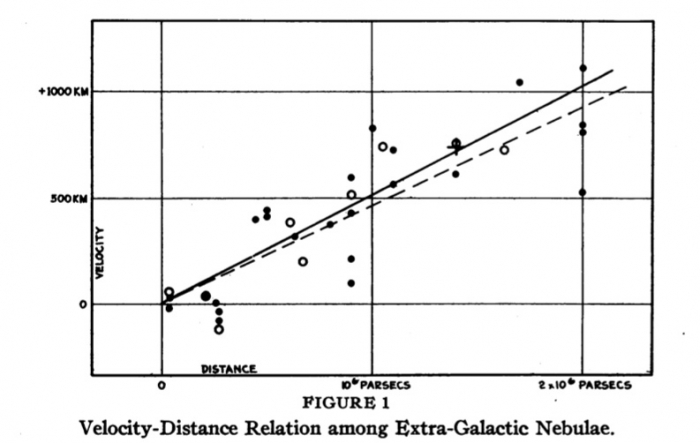
\includegraphics[width=\textwidth]{hubbleslaw}
        \caption{Hubbles Law}
        \label{fig:hubbleslaw}
\end{figure}

The observed \emph{redshifts} couldn't be explained by the proper motion of
the galaxies, instead this phenomenon was caused by the continuos expansion
of our universe.

An expanding universe was first theorized by Friedmann in 1922, before Hubble's
observations, as a consequence of the field equations of the theory of the
\emph{General Relativity} (GR). The starting point of Friedmann derivation was
an elegant and powerful assumption about the structure of our universe:
the \emph{Cosmological Principle}.

\subsection{The Cosmological Principle}\label{ss:cosmological_principle}

The matter in the universe we observe is clustered in gravitationally bound
structures, but observations at large scale (\SI{> 100}{\mega\parsec}) shows
that the place we call home appears to obey the \emph{Cosmological
Principle}:

\begin{principle}[Cosmological Principle]
        On the largest scales, the universe is spatially homogeneous and isotropic.
\end{principle}

Note that this principle is valid for every possible observer in the
universe. We see an homogeneous and isotropic universe from our planet, and
we believe that any other observer in the universe does: there's no special
place in our universe.

There are two main piece of evidence for the cosmological principle:

\begin{itemize}
        \item The \emph{Comsmic Microwave Background Radiation} (CMB): an almost
        uniform sea of photons which fills all space and provides a snapshot of the
        universe at \num{\sim 380000} years after its birth. The CMB
        presents small fluctuations in temperature with a characteristic
        scale:

        \begin{equation}
                \frac{\var{T}}{T} \sim \num{e-5}
        \end{equation}

        \item A relevant number of \emph{redshift surveys} show that the
        distribution of stars looks increasengly smooth on larger scales.
\end{itemize}

The acceptance of such a profound statement it's the prologue to the
description of the geometry of \emph{spacetime}.

\subsection{The FLRW Metric}\label{ss:flrw}

Friedmann, Lema\^itre, Robertson and Walker during the 1920-1930s proved
independently that the most generic metric based on the cosmological
principle is the Friedmann-Lema\^itre-Robertson-Walker (FLRW) metric:

\begin{equation}
        \dd{s}^2 = -c^2\dd{t^2} + a\qty(t)^2\qty[\dd{\chi}^2 +
        f_k\qty(\chi)^2\dd{\Omega}^2]
        \label{eq:flrw}
\end{equation}

Where:

\begin{itemize}
        \item $c$ is the speed of light in vacuum;
        \item $a\qty(t)$ is a real function of time known as \emph{scale factor};
        \item $k$ is a real number which parametrizes the spatial curvature of the
        spacetime. Due to the homogeneity and isotropy of space, $k$ is at most a
        function of time. For a fixed time $k$ is a constant and:

        \begin{itemize}
                \item $k = 0$ $\rightarrow$ flat universe;
                \item $k > 0$ $\rightarrow$ open universe;
                \item $k < 0$ $\rightarrow$ closed universe.
        \end{itemize}

        in particular:

        \begin{equation}
                f_k\qty(\chi) =
                        \begin{cases}
                                 \chi & \qif k = 0 \\
                                 \sqrt{k}^{-1} \sin(\sqrt{k} \chi) & \qif k > 0 \\
                                 \sqrt{\abs{k}}^{-1} \sinh(\sqrt{\abs{k}} \chi) & \qif k < 0
                        \end{cases}
        \end{equation}
        \item and $\dd{\Omega}^2 = \dd{\theta}^2 + \sin[2](\theta) \dd{\phi}^2$
        is the metric of the unitary sphere.
\end{itemize}

The FLRW metric in \autoref{eq:flrw} is invariant under the following transformation:

\begin{equation}
        \begin{split}
                \chi & \rightarrow \frac{\chi}{\lambda} \\
                k & \rightarrow \lambda k \\
                a & \rightarrow \lambda a
        \end{split}
\end{equation}

so it is possible to set:

\begin{align}
k & = 0,\pm 1 \\
a\qty(t_0) & = 1
\end{align}

where $t_0$ is the present time and the function $f_k$ becomes:

        \begin{equation}
                f_k\qty(\chi) =
                        \begin{cases}
                                 \chi & \qif k = 0 \\
                                 \sin \chi & \qif k = 1 \\
                                 \sinh \chi & \qif k = -1
                        \end{cases}
        \end{equation}

We can immediately note that the valid geometry for an homogeneous
and isotropic spacetime are either flat, spherical or hyperbolic.

\subsection{The Comoving Distance and the Hubble Parameter}

Consider two points in a slice of space in the spacetime ($t = t_*$): $p_1$,
$p_2$. The physical distance between them is calculated using the FLRW
metric for a fixed time:

\begin{equation}
        \dd{s} = a\qty(t_*)\sqrt{\dd{\chi}^2 +
        f_k^2\qty(\chi)\dd{\Omega}^2}
\end{equation}

integrating between $p_1$ and $p_2$, we obtain:

\begin{equation}
        d_{\text{phys}} = a\qty(t_*)d_{\text{co}}
        \label{eq:dd}
\end{equation}

where $d_{\text{co}}$ is the comoving distance, the distance in comoving
coordinates, which expand in the same way as space, and $d_\text{phys}$ is
the proper or physical distance.

Taking the time derivative of \autoref{eq:dd}:

\begin{equation}
        v_{\text{phys}} = \dot a\qty(t) d_{\text{co}} = \frac{\dot a\qty(t)}{a\qty(t)} d_{\text{phys}}
\end{equation}

where $v_{\text{phys}}$ is the physical or proper velocity and the function:

\begin{equation}
        H\qty(t) = \frac{\dot a\qty(t)}{a\qty(t)}
        \label{eq:hubble_parameter}
\end{equation}

is called the \emph{Hubble parameter} and its present day value $H\qty(t_0)
\equiv H_0$ is the \emph{Hubble's constant}, introduced in
\autoref{ss:hubbleslaw}. The Hubble's constant is a cosmological
parameter of our standard cosmological model and has a positive value,
indicating that we live in an expanding universe.

\subsection{The Dynamics of Spacetime}

The evolution of the scale factor $a$ introuced in \autoref{ss:flrw} is
governed by Einstein field equations of GR:

\begin{equation}
        G_{\mu \nu} = \frac{8 \pi G}{c^2} T_{\mu \nu}
        \label{eq:einstein}
\end{equation}

where:

\begin{itemize}
        \item $G_{\mu \nu}$ is the Einstein tensor, which describes the
        geometry of the spacetime;
        \item $G$ is the universal gravitational constant;
        \item $T_{\mu \nu}$ is the energy-momentum tensor, responsible for
        the energy and momentum of matter.
\end{itemize}

Einstein fields equations of GR relate the geometry of the spacetime to the
distribution of matter within it. Assuming the cosmological principle, we
can choose $T_{\mu \nu}$ to be the energy-momentum tensor of a perfect
fluid, which can be completely characterized by its density and pressure:

\begin{equation}
         T_{\mu \nu} = (\rho c^2 + P)u_\mu u_\nu + P g_{\mu \nu}
         \label{eq:energy_momentum_tensor}
\end{equation}

Substituting \autoref{eq:flrw} and \autoref{eq:energy_momentum_tensor} in
\autoref{eq:einstein}, the field equations reduces to two equations for the
time evolution of the scale factor, known as \emph{Friedmann equations} and
written by Friedmann himself in 1922:

\begin{align}
        \qty(\frac{\dot a\qty(t)}{a\qty(t)})^2 & = \frac{8\pi G}{3} \rho\qty(t)
        - \frac{k\qty(t) c^2}{a^2\qty(t)}
        \label{eq:friedmann_1} \\
        \frac{\ddot a\qty(t)}{a\qty(t)} & = -\frac{4\pi G}{3}
        \qty(\rho\qty(t) + \frac{3 P\qty(t)}{c^2})
        \label{eq:friedmann_2}
\end{align}

The Friedmann equations constitutes a system of two differential equations
with three variables quantity: $a\qty(t)$, $\rho\qty(t)$ and $P\qty(t)$.
The last equation we need to close the system can be deduced from the
conservation of the energy-momentum tensor:

\begin{equation}
        \partial_\mu T^{\mu \nu} = 0
\end{equation}

It's the \emph{continuity equation}, which express the conservation of energy in a
comsmological setting:

\begin{equation}
        \dot \rho + 3 H \qty(\rho + \frac{P}{c^2}) = 0
        \label{eq:continuity}
\end{equation}

A state equation of the kind $P = P\qty(\rho)$ can be specified to
integrate the continuity equation and determine how the energy density
depends on the scale factor. We guess a generic and simple shape for the
state equation of each component of the cosmological fluid:

\begin{equation}
        P = w \rho c^2
        \label{eq:state}
\end{equation}

where $w$ is a parameter typical of each component.
Using \autoref{eq:state} in \autoref{eq:continuity} we obtain:

\begin{equation}
        \frac{\dot \rho}{\rho} = -3\qty(1 + w) \frac{\dot a}{a}
\end{equation}

integrating over time from $t_0$ to a generic time $t$ and using the fact
that $a\qty(t_0) = 1$:

\begin{equation}
        \rho_w\qty(t) = \rho_{w,0} a^{-3\qty(1 + w)}
\end{equation}

where $\rho_{0,w}$ is the present day energy density.
Therefore the total energy density for the cosmological fluid is:

\begin{equation}
        \rho_{\text{tot}} = \sum_w \rho_w
\end{equation}

and \autoref{eq:friedmann_1} becomes:

\begin{equation}
        H^2\qty(t) = \frac{8\pi G}{3} \rho_{\text{tot}}\qty(t) -
        \frac{k\qty(t) c^2}{a^2\qty(t)}
\end{equation}

where we have used \autoref{eq:hubble_parameter}. The curvature parameter
$k$ can isolated in the right-hand side of the equation:

\begin{equation}
        \begin{split}
                \frac{k\qty(t) c^2}{a^2\qty(t)} & =
                \frac{8\pi G \rho_{\text{tot}}\qty(t)}{3} - H^2\qty(t) \\
                \frac{k\qty(t) c^2}{a^2\qty(t)} & =
                H^2\qty(t) \qty(\frac{8\pi G \rho_{\text{tot}}\qty(t)}{3H^2\qty(t)} - 1) \\
                k(t) & = \frac{H^2\qty(t) a^2\qty(t)}{c^2} \qty(\Omega\qty(t) - 1) \\
        \end{split}
        \label{eq:friedmann_curvature}
\end{equation}

In the last equation we have defined:

\begin{align}
        \rho_c\qty(t) & \equiv \frac{3H^2\qty(t)}{8\pi G} \\
        \Omega\qty(t) & \equiv \frac{\rho_{\text{tot}}\qty(t)}{\rho_c\qty(t)}
\end{align}

The function $\rho_c\qty(t)$ is known as the \emph{critical density}: it
represents the energy density time evolution for a flat universe ($k = 0$).
We note that in this case, the total energy density of the universe is
directly related to the Hubble parameter.

Evaluating \autoref{eq:friedmann_curvature} for $t = t_0$ and assuming a
time independent space curvature $k(t) = k$, yields:

\begin{equation}
        k = \frac{H^2_0}{c^2} \qty(\Omega_0 - 1) \\
\end{equation}

where:

\begin{equation}
        \Omega_0 \equiv \frac{\rho_0}{\rho_{c,0}} = \sum_w
        \frac{\rho_{w,0}}{\rho_{c,0}} \equiv \sum_w \Omega_w
\end{equation}

The adimensional quantities $\Omega_w$ are the \emph{density parameters}
for each fluid component. Note that even though we have omitted the $0$
subscript, the density parameters refer to the fraction of energy observed
today, as the definition implies.

The density parameters sum to:

\begin{equation}
        \sum_w \Omega_w = 1 + \frac{kc^2}{H^2_0}
\end{equation}

as a consequence, if we live in a flat universe then we must have $\sum_w
\Omega_w = 1$. Any excess energy density, with $\sum_w \Omega_w > 1$ means
that we necessarily live in a positively curved universe with $k = +1$. Any
deficit in energy, with $\sum_w \Omega_w < 1$ gives rise to a negatively
curved $k = 1$ universe. Measuring the present day total energy density
$\rho_{\text{tot},0}$ and the Hubble constant $H_0$, gives us the
opportunity to have knowledge of the spatial geometry of our universe.

\subsection{The Components of the Cosmological Fluid}

According to current theories and pieces of evidence, there are three
entities that contribute to the current energy density of our universe:

\begin{itemize}
        \item Conventional matter or \emph{dust};
        \item Radiation;
        \item Dark Energy or \emph{cosmological constant}.
\end{itemize}

To derive a solution for the time evolution of the scale factor $a\qty(t)$
in our universe, it is essential to write a state equation
$P\qty(\rho) = \rho$ for each one of these component:

\begin{itemize}
        \item For dust-like matter (e.g. galaxies or cold dark matter):
        $P_m\qty(\rho_m) = 0$;
        \item For radiation we must impose a null trace for the energy-momentum
        tensor $T_{\mu \nu}$ in \autoref{eq:energy_momentum_tensor}: $P_r\qty(\rho_m)
        = \frac{1}{3} \rho_r c^2$;
        \item For Dark Energy the equation of state is obtained
        substituting  $G_{\mu \nu} = -g_{\mu \nu} \Lambda$, with $\Lambda =
        \text{const.}$ and $\Lambda > 0$, in \autoref{eq:einstein}:
        $P_\Lambda\qty(\rho_\Lambda) = -\rho_\Lambda c^2$, $\rho_\Lambda =
        \frac{\Lambda}{8\pi G}$.
\end{itemize}

The dependence on the scale factor for the energy densities characterized by
these state equations is found making use of the continuity equation
(\autoref{eq:continuity}):

\begin{align}
        \rho_m\qty(a) & = \rho_{m,0}a^{-3} \label{eq:rho_m} \\
        \rho_r\qty(a) & = \rho_{r,0}a^{-4} \label{eq:rho_r} \\
        \rho_\Lambda\qty(a) & = \rho_{\Lambda,0} \label{eq:rho_lambda} \\
\end{align}

The quantity $\Lambda$ is known as the \emph{cosmological constant} and the
corresponding density $\rho_\Lambda$ is the \emph{vacuum energy density},
associated with the \emph{zero-point energy} of the vacuum state. Note that
Dark Energy has negative pressure $P_\Lambda = -\rho_\Lambda c^2$, and it
does not dilute away as the universe expands.

The total energy density of our universe is:

\begin{equation}
        \rho_\text{tot}\qty(a) = \frac{\rho_{m,0}}{a^3} + \frac{\rho_{r,0}}{a^4} +
        \rho_{\Lambda,0}
\end{equation}

An expanding universe is radiation dominated at first, in a second phase
its expansion is driven by matter and at last by Dark Energy. In fact every
universe characterized by a non-zero cosmological constant ($\Lambda \neq
0$) will be ultimately become dodinated by the vacuum energy density
$\rho_\Lambda$. A plot of the evolution of the three kinds of energy
density is shown in \autoref{fig:density_evolution}.

\begin{figure}
        \centering
        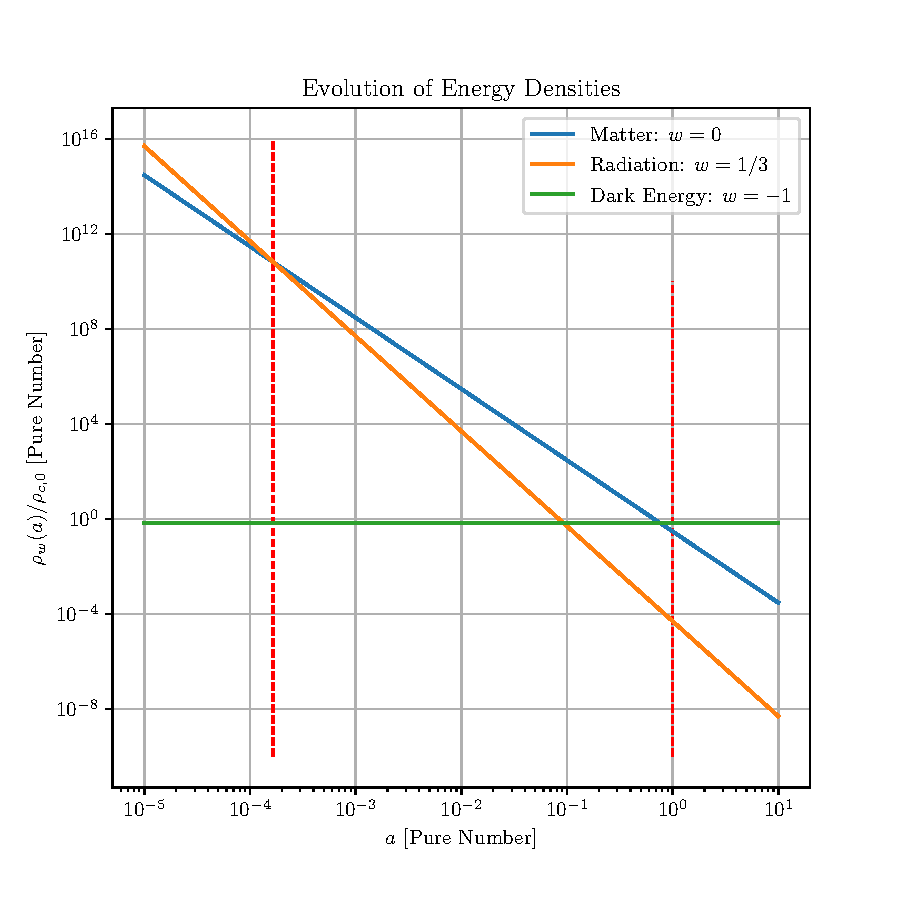
\includegraphics[width=\textwidth]{density_evolution}
        \caption{Energy density evolution.}
        \label{fig:density_evolution}
\end{figure}

Given the total energy density we can solve the first Friedmann equation
and obtain the evolution of the scale factor in our universe. The scale
factors for the three different space curvatures ($k = 0,\pm 1$) in the
simple case of a matter dominated universe are sketched in
\autoref{fig:scale_factor_evolution_matter}. In the case of an expanding
flat or hyperbolic geometry ($k = 0,-1$) the universe expands for ever with:

\begin{equation}
        \dot a\qty(t \rightarrow +\infty)
                \begin{cases}
                        > 0 & \qif k = -1 \\
                        \rightarrow 0 & \qif k = 0
                \end{cases}
\end{equation}

The spherical universe ($k = +1$) instead eventually re-collapses at a finite
time $t_{\text{bc}}$ with:

\begin{equation}
        a\qty(t_{\text{bc}}) = 0
\end{equation}

This event is known as \emph{Big Crunch}.

\begin{figure}
        \centering
        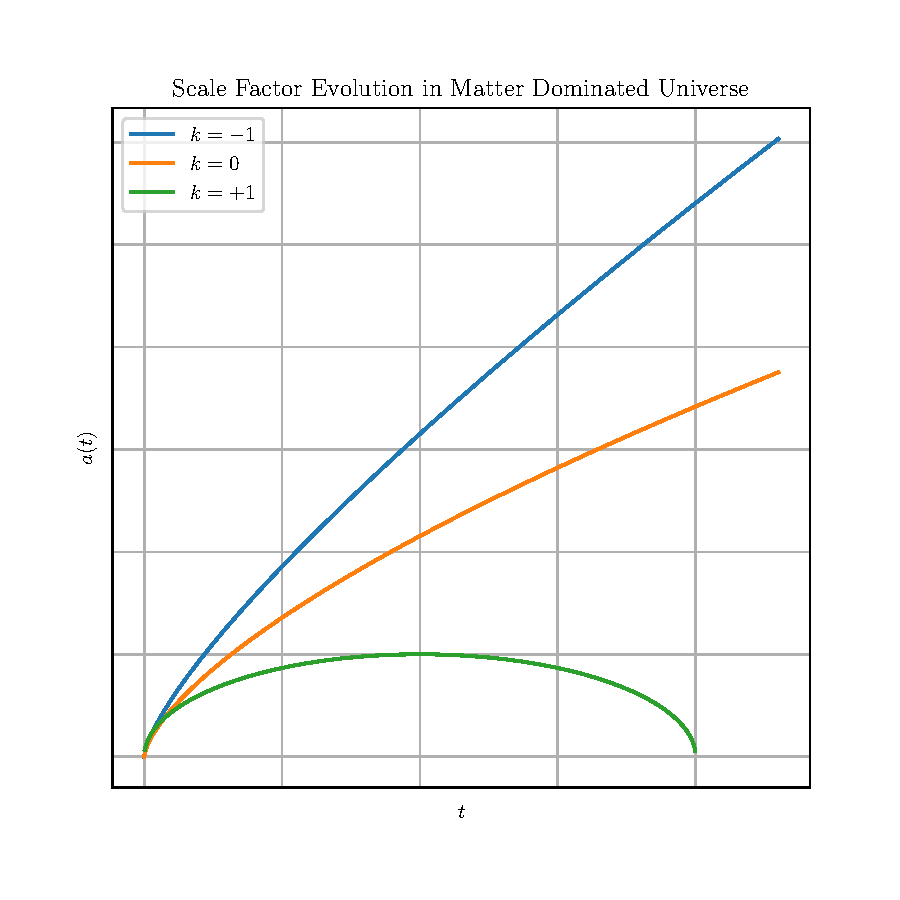
\includegraphics[width=\textwidth]{scale_factor_evolution_matter}
        \caption{Scale factor evolution in a matter dominated universe.}
        \label{fig:scale_factor_evolution_matter}
\end{figure}

In the case of Dark Energy dominated universe every possible solution for
each one of the three space curvatures describes the same spacetime, but with
different coodinates. This spacetime is kwown as \emph{de Sitter space}.
The evolution of the scale factor for this kind of universe is shown in
\autoref{fig:scale_factor_evolution_sitter}. This solution shows a
contracting phase when $t < 0$, followed by a phase of accelerating
expansion ($\ddot a > 0$) when $t > 0$. In particular there's no
\emph{Big Bang} when $t = 0$:

\begin{equation}
        a\qty(t = 0) = \sqrt{\frac{3c^2}{\Lambda}}
\end{equation}

\begin{figure}
        \centering
        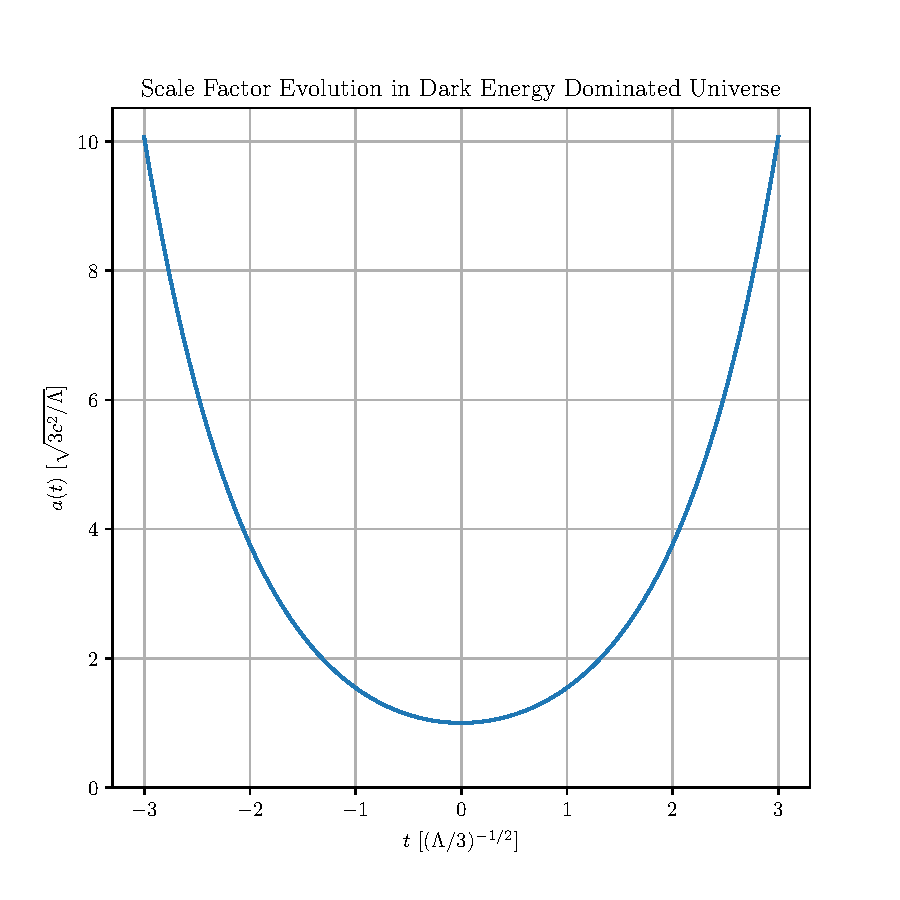
\includegraphics[width=\textwidth]{scale_factor_evolution_sitter}
        \caption{Scale factor evolution for de Sitter space}
        \label{fig:scale_factor_evolution_sitter}
\end{figure}

\subsection{The \texorpdfstring{$\Lambda$}{LAMBDA-}CDM Cosmological Model}

Substituting the expressions for the energy densities of the components of
the cosmological fluid (\autoref{eq:rho_m}, \autoref{eq:rho_r} and
\autoref{eq:rho_lambda}) in \autoref{eq:friedmann_1} yields the second
Friedmann equation for our universe:

\begin{equation}
        H^2\qty(t) = \frac{8\pi G}{3} \qty(\frac{\rho_{m,0}}{a^3\qty(t)} +
        \frac{\rho_{r,0}}{a^4\qty(t)} + \rho_{\Lambda,0}) -
        \frac{k\qty(t) c^2}{a^2\qty(t)}
\end{equation}

If the first term in the right-hand side is multiplied and
divided by the squared hubble constant $H^2_0$, the equation is parametrized
by the density parameters $\Omega_w$:

\begin{equation}
        H^2\qty(t) = H^2_0 \qty(\frac{\Omega_m}{a^3\qty(t)} +
        \frac{\Omega_r}{a^4\qty(t)} + \Omega_\Lambda) -
        \frac{k\qty(t) c^2}{a^2\qty(t)}
\end{equation}

The collection of the numbers $\Omega_m$, $\Omega_r$, $\Omega_\Lambda$ and
$k$ goes by the name of the \emph{$\Lambda$CMD model}, with $\Lambda$
denoting the cosmological constand and CMD denoting \emph{cold dark matter}.
The great interest in the study of the Cosmic Microwave Background resides
in the fact that the values of the parameters of the $\Lambda$CMD
cosmological model can be extracted from observations of this relic
radiation.

\section{The CMB Radiation}

This section is devoted to the introduction of the Comsmic Microwave
Background (CMB) Radiation. To understand what caused the CMB radiation to
emerge, we start describing what we think happened in the universe from the
first instants after the Big Bang to today.

\subsection{A Brief Thermal History of Our Universe}\label{ss:brief_thermal_history}

The essence of the hot Big Bang theory is simply to go back in time taking
the temperature scaling $T \sim \frac{1}{a}$. As the solution for the scale
factor suggests, as we go further back in time, more the temperature and
the energy density of the universe increase and more species join the
primordial plasma reaching the thermodinamic equilibrium. As we know in the
early stages the universe was radiation dominated, so the temperature and
energy density decreased according to:

\begin{equation}
        T\qty(t), \rho\qty(t) \propto t^{-\frac{1}{2}}
\end{equation}

A summary of some of the key events in the early history of the universe
follows:

\begin{itemize}
        \item \textbf{Electroweak phase transition:} \SI{e-12}{\second},
        \SI{e22}{\kelvin}

        At this time the electroweak phase transition occured, separating
        the weak and electromagnetic interactions. In this epoch the
        universe was filled with a quark-gluon plasma.
        \item \textbf{QCD phase transition:} \SI{e-6}{\second},
        \SI{e16}{\kelvin}

        At this time the average energy of particles interaction had fallen
        below the mass of the adrons. In this epoch the temperature was
        high enough that hadrons and anti-hadrons pairs could form. Later
        new pairs were no longer produced and most of the hadrons and
        anti-hadrons annihilated. Due to the matter and anti-matter
        assimmetry a small portion of hadrons remained in the universe.

        At this time the universe was filled with neutrons and protons in
        the ratio of:

        \begin{equation}
                \frac{n_n}{n_p} = \frac{1}{5}
        \end{equation}

        due to the small mass difference between the two particles. Later
        this ratio became smaller as a consequence of the neutron $\beta$
        decay:

        \begin{equation}
                n \rightarrow p + e^- + \bar\nu_e
        \end{equation}

        and its present day value is:

        \begin{equation}
                \frac{n_n}{n_p} = \frac{1}{7}
        \end{equation}

        \item \textbf{Neutrino Decoupling:} \SI{1}{\second},
        \SI{e10}{\kelvin}

        At this time neutrinos decoupled from the primordial plasma and
        began to travel freely into space. As neutrinos rarely interact
        with matter, they still exist today as the Cosmic
        Neutrino Background (C$\nu$B), analogous to the much later Cosmic
        Microwave Background emitted during recombination.

        \item \textbf{$e^-e^+$ Annihilation:} \SI{6}{\second},
        \SI{5e9}{\kelvin}

        At this time the average energy of photons became less then the rest mass
        of the electron-positron pairs and the reaction:

        \begin{equation}
                2\gamma \rightleftharpoons e^- + e^+
        \end{equation}

        fell out of equilibrium. The left $e^-e^+$ pairs annihilated and,
        due to the matter and anti-matter asimmetry, just a small portion
        of electrons survived.

        \item \textbf{Nucleosynthesis:} \SI{3}{\minute}, \SI{e9}{\kelvin}

        At this time the tempearture and pressure of the universe allowed
        the stabilization of deuterium and the consequent formation of
        light nuclei, such as hydrogen and its isotopes
        (\SI{\sim 75}{\percent}) and helium (\SI{\sim 25}{\percent}).

        \item \textbf{Matter-Radiation Equality:} \SI{50000}{\year},
        \SI{8700}{\kelvin}

        At this time the universe became matter dominated: the energy
        density of matter $\rho_m$ became equal to the energy density of
        radiation $\rho_r$ (\autoref{fig:density_evolution}).

        \item \textbf{Recombination and Last Scattering:} \SI{370000}{\year},
        \SI{3000}{\kelvin}

        At this time the universe has cooled enough ($k_bT <<
        \SI{13.6}{\electronvolt}$) to allow the formation of the first
        neutral atoms. This event is known as \emph{recombination} and it is
        associated to the photons decoupling or \emph{last scattering}, that
        refers to the mean free path of photons in the universe becoming
        infinite. Nowadays the last scattering photons are still propagating in
        space and we refer to them as the \emph{Cosmic Microwave Background}.

        \item \textbf{Matter-Dark Energy Equality:} \SI{e10}{\year},
        \SI{3.8}{\kelvin}

        At this time the universe became dominated by Dark Matter: the
        vacuum energy density $\rho_\Lambda$ became equal to the energy density of
        matter $\rho_m$ (\autoref{fig:density_evolution}), determining a
        phase of accelerated expansion.

        \item \textbf{Today:} \SI{1.38e10}{\year}, \SI{2.7}{\kelvin}

        The epoch we live in.
\end{itemize}

\subsection{The First Revelation of the CMB}

The Cosmic Microwave Background was first predicted in 1984 by Ralph Alpher
and Robert Herman, who also provided a first estimation of its brightness
temperature (\SI{\sim 5}{\kelvin}).

Andrew McKellar in 1941 used spectroscopic observations of the cyano radical
absorpsion lines in star spectra to detect a rotational temperature of
interstellar molecules. However McKellar failed to provide a cosmological
interpartation for these observations.

In 1964 Arno Penzias and Robert Wilson were working at Bell Laboratories
on a microwave horn antenna (\autoref{fig:horn_antenna_pw}) originally used by
the Bell telephone companies for satellite communication.
To their surprise they found a background noise which did not depend on the
direction, with a temperature that they measure to be between
\SI{2.5}{\kelvin} and \SI{4.5}{\kelvin}. They were observing the CMB
radiation and for this discovery they were awarned the Nobel Prize in 1978.

\begin{figure}
        \centering
        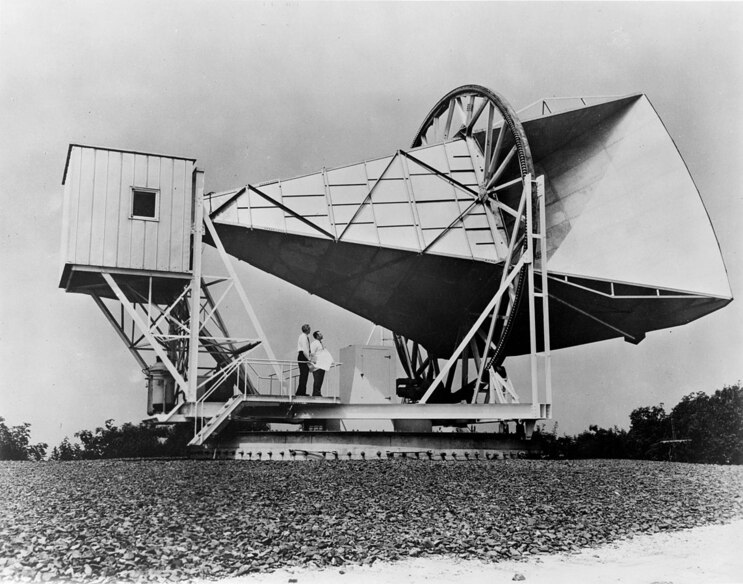
\includegraphics[width=\textwidth]{Horn_Antenna_PW}
        \caption{Penzias and Wilson's microwave horn antenna.}
        \label{fig:horn_antenna_pw}
\end{figure}

\subsection{The CMB Black Body Spectrum}

Just before recombination and last scattering photons were
coupled with matter and in thermodinamic equilibrium. The spectral density
of electromagnetic radiation in thermodinamic equilibrium is described by
the \emph{Planck law}:

\begin{equation}
        B_\nu\qty(T) = \frac{2h\nu^3}{c^2}
        \frac{1}{\exp(\frac{h\nu}{K_b T}) - 1}
\end{equation}

where $T$ is the temperature of the thermal bath, $\nu$ is the frequency of
the electromagnetic radiation, $K_b$ is the Boltzmann constant and $h$ is
the quantum of action, the Planck constant. As mentioned in
\autoref{ss:brief_thermal_history}, at recombination the temperature of the
universe was \SI{\sim 3000}{\kelvin}, therefore, making use of the Wien
Law:

\begin{align}
        \lambda_{\text{peak}} & = \frac{b}{T} \\
        b & \approx \SI{2.897e-3}{\meter\kelvin}
\end{align}

where $\lambda_{\text{peak}}$ is the wavelength at which the spectrum
peaks, we know that at recombination:

\begin{equation}
        v_{\text{CMB,max}} \approx \SI{7e4}{\giga\hertz}
\end{equation}

As we stated in \autoref{ss:brief_thermal_history}, the temperature of the
universe is related to the scale factor

\begin{equation}
        T\qty(a) \propto \frac{1}{a}
\end{equation}

and as a consequence

\begin{equation}
        T\qty(a_0) = T\qty(a_{\text{rec}}) a_{\text{rec}}
        \label{eq:t_scale}
\end{equation}

where $a_{\text{rec}}$ is the scale factor at the time of recombination.

At the same time, the photons of the CMB radiation are affected by \emph{cosmological
redshift}, due to Universe expansion. The wavelenght of the light emitted
at the time of recombination differs from the light observed at present
time, according to the law

\begin{equation}
        \lambda\qty(a_0) = \frac{\lambda\qty(a_{\text{rec}})}{a_{\text{rec}}}.
\end{equation}

For frequency this translates to

\begin{equation}
        \nu\qty(a_0) = \nu\qty(a_{\text{rec}}) a_{\text{rec}}
        \label{eq:nu_scale}
\end{equation}

and, if we combine \autoref{eq:t_scale} and \autoref{eq:nu_scale}, we
obtain:

\begin{equation}
        \frac{h \nu\qty(a_0)}{K_b T\qty(a_0)} =
        \frac{h \nu\qty(a_{\text{rec}})}{K_b T\qty(a_{\text{rec}})}.
\end{equation}

This last equation asserts that the shape of the CMB spectrum does not
change as the Universe expands. However, the characteristic temperature and
peak frequency of the spectrum have changed according to
\autoref{eq:t_scale} and \autoref{eq:nu_scale}, so that

\begin{align}
        T_{\text{CMB}} & \approx \SI{3000}{\kelvin} a_{\text{rec}} \approx
        \SI{3}{\kelvin} \\
        v_{\text{CMB,max}} & \approx \SI{7e4}{\giga\hertz} a_{\text{rec}}
        \approx \SI{70}{\giga\hertz}
\end{align}

The spectrum of the CMB was measured with high accuracy
(see \autoref{fig:cmb_spectrum_cobe})
by the \emph{Far infrared Absolute Spectrometer} (FIRAS) instrument onboard
the \emph{Cosmic Background Explorer} (COBE) satellite: it is a near
perfect blackbody spectrum at $T = \SI{2.7260 \pm 0.0013}{\kelvin}$

\begin{figure}
        \centering
        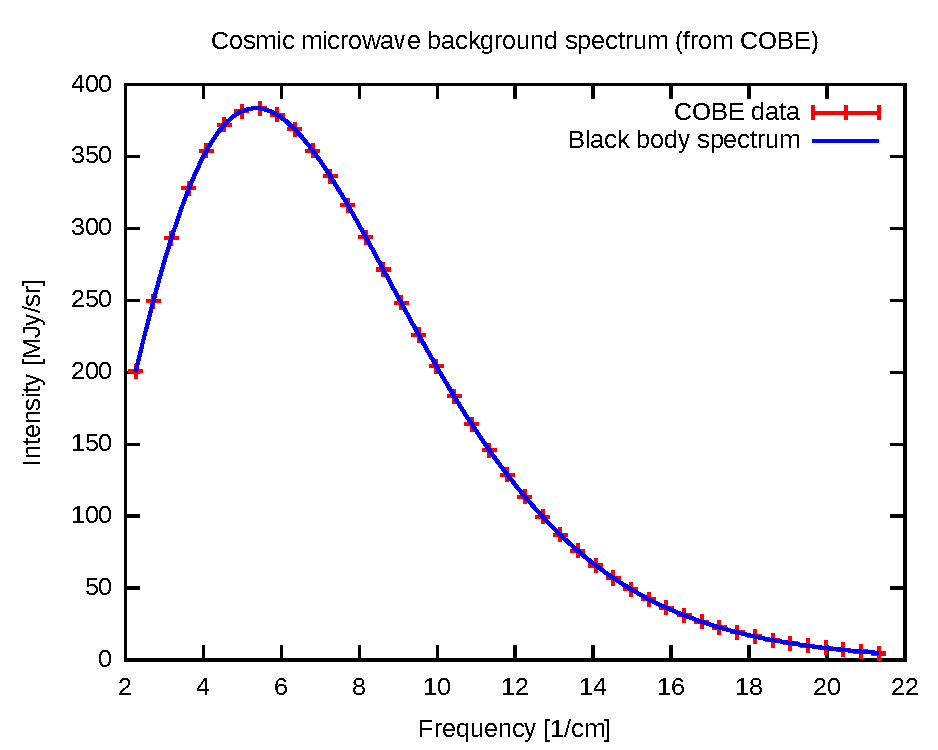
\includegraphics[width=\textwidth]{CMB_Spectrum_COBE}
        \caption{CMB Spectrum COBE}
        \label{fig:cmb_spectrum_cobe}
\end{figure}

\section{The CMB Temperature Anisotropies}

The CMB radiation is extremely isotropic. As mentioned in
\autoref{ss:cosmological_principle} the temperature anisotropies are of the
order of

\begin{equation}
\frac{\Delta T\qty(\theta,\phi)}{\bar T} \sim \num{e-5}
\end{equation}

for every $\theta$ and $\phi$ on the sky, $0 \leq \theta \leq \pi$,
$0 \leq \phi \leq 2\pi$.

Sachs and Wolfe in 1967 had theorized first the presence of temperature
anisotropies in the CMB spectrum at large angular scales. Later
anisotropies were linked to the quantum oscillations in primordial plasma,
but the instruments used before the 90s were not sensible enough to carry
out useful measures of this phenomenon.

The \emph{Differential Microwave Radiometer} (DMR) instrument onboard the
COBE satellite was the first experiment to map the CMB temperature
anisotropies.The instrument consists of six differential microwave
radiometers, two nearly independent channels that operate at each of three
frequencies: \SI{ 31.5}{\giga\hertz}, \num{53}, and \SI{90}{\giga\hertz}.
Making use of two years of DMR data, the amplitude of temperature fluctuations
was reported to be
\SI{36 \pm 5}{\micro\kelvin} at \ang{7}, and
\SI{30.5 \pm 2.7}{\micro\kelvin} when smoothed to \ang{10}.
The sky maps obtained by DMR is showed in \autoref{fig:dmr_maps}.

\begin{figure}
        \centering
        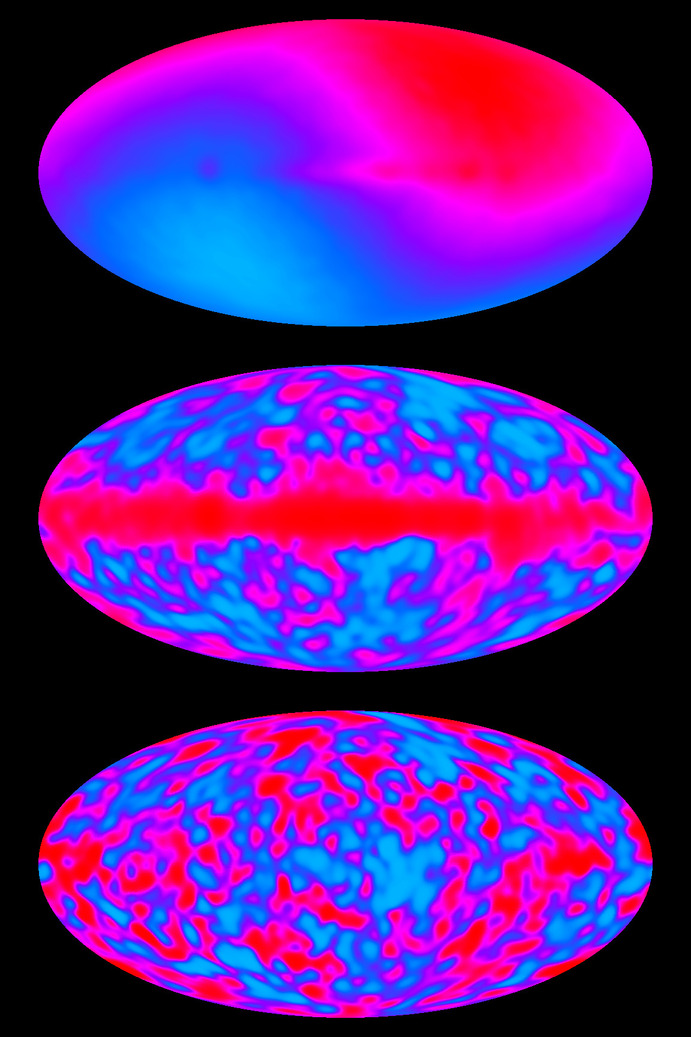
\includegraphics[width=0.80\textwidth]{DMR_maps}
        \caption{The following image is similar to the June 1992 Physics
        Today cover picture, with the map including the dipole and Galaxy
        on the top, the dipole removed map in the middle, and the reduced
        map on the bottom. The dipole, a smooth variation between
        relatively hot and relatively cold areas from the upper right to
        the lower left, is due to the motion of the solar system relative
        to distant matter in the universe. The signals attributed to this
        variation are very small, only one thousandth the brightness of the
        sky.}
        \label{fig:dmr_maps}
\end{figure}

The second generation of CMB experiments was represented by the
\emph{Wilkinson Microwave Anisotropy Probe} (WMAP). The WMAP mission was
designed to acquire a \ang{;13;} FWHM resolution full sky
map of the temperature anisotropy of the cosmic microwave background
radiation. WMAP observed the microwave sky for \num{9} years in \num{5}
bands. The skymap data products derived from the WMAP observations have
\num{45} times the sensitivity and \num{33} times the angular resolution
of the COBE-DMR mission.

\emph{Planck} was the third generation of space-based cosmic microwave background
experiments, after NASA's COBE and NASA's WMAP. It was also the third
Medium-Sized Mission (M3) of European Space Agency's (ESA's) Horizon 2000
Scientific Program. The basic scientific goal of the Planck mission is to
measure CMB anisotropies at all angular scales larger than \ang{;10;}
over the entire sky with a precision of \num{\sim 2} parts per million.
The model payload consisted of a \SI{1.5}{\meter} off-axis telescope with
two focal plane arrays of detectors sharing the focal plane. Low frequencies
were covered by \num{56} tuned radio receivers sensitive to
\SIrange{30}{100}{\giga\hertz}, while high frequencies were be covered by
\num{56} bolometers sensitive to \SIrange{100}{850}{\giga\hertz}.
The Planck mission permitted the extraction of the most precise map of the
CMB temperature anisotropies, to date. This map is depicted in
\autoref{fig:planck_cmb}.

\begin{figure}
        \centering
        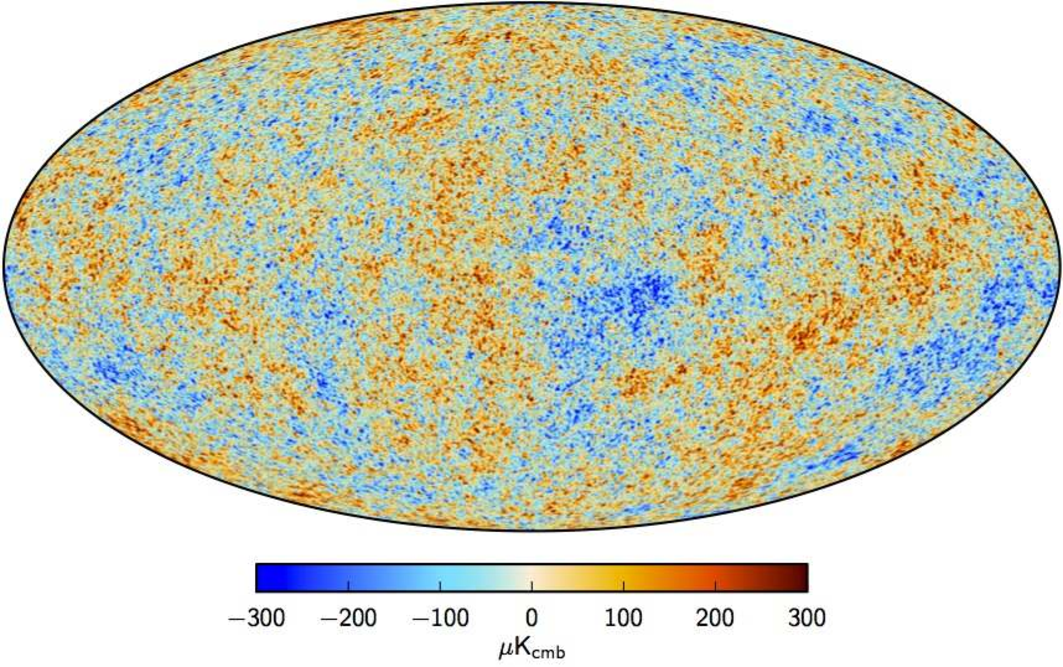
\includegraphics[width=\textwidth]{Planck_CMB}
        \caption{CMB Anisotropies Planck}
        \label{fig:planck_cmb}
\end{figure}

A comparison of the results obtained by COBE, WMAP, and Plank is showed in
\autoref{fig:cobe_wmap_planck_comparison}.

\begin{figure}
        \centering
        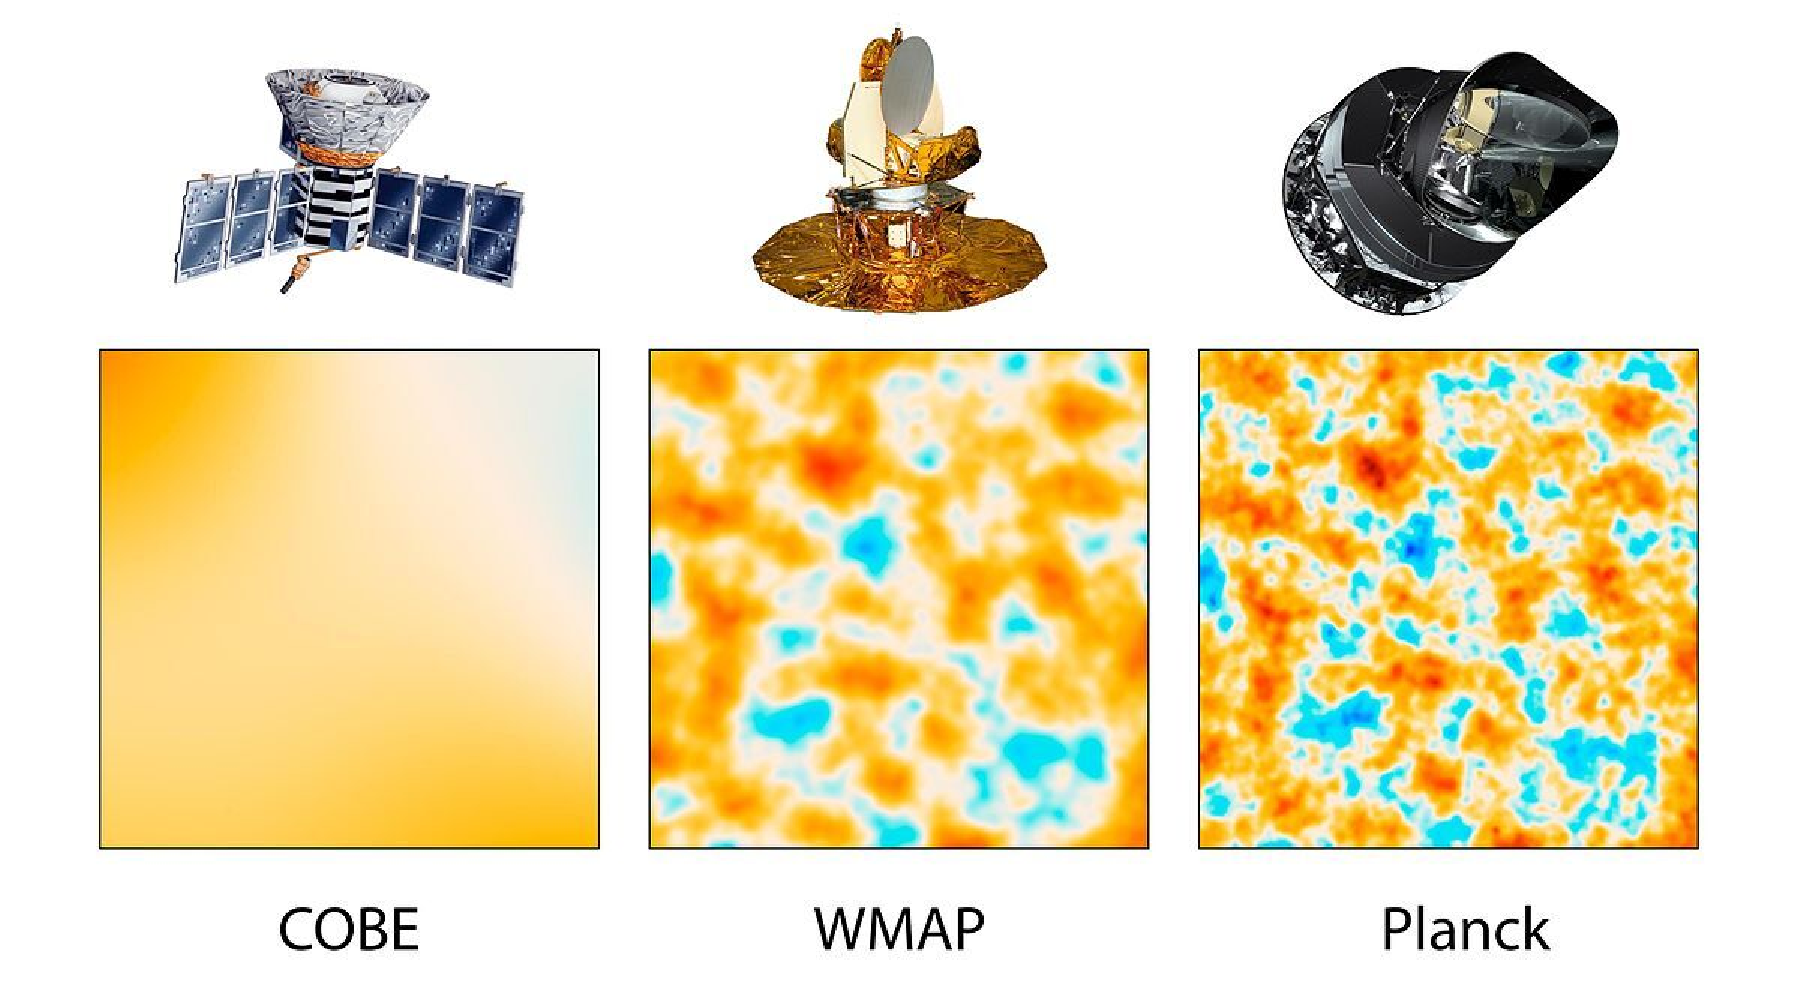
\includegraphics[width=\textwidth]{cobe_wmap_planck_comparison}
        \caption{COBE, WMAP, and Plank results comparison.}
        \label{fig:cobe_wmap_planck_comparison}
\end{figure}

\subsection{Density Fluctuations}

The CMB radiation anisotropies contain an imprint of the anisotropies at
the time of recombination and, if traced back in time, they can be
interpreted as a signature of the perturbations in the primordial plasma.
Precise measures of the CMB anisotropies pattern let us discriminate
between different cosmological models.

The perturbations in the early universe were adiabatic, that is, the
perturbations in all components of the cosmological fluid are proportional.
In particular

\begin{equation}
        \delta_r\qty(\vb{\chi},t) \equiv \frac{4}{3} \delta_m\qty(\vb{\chi},t)
\end{equation}

where $\delta_x\qty(\vb{\chi},t)$ is the \emph{density contrast} for a
specific component of the cosmological fluid

\begin{equation}
        \delta_x\qty(\vb{\chi},t) = \frac{\var{\rho_x\qty(\vb{\chi},t)}}{\bar \rho_x}
\end{equation}

$\bar \rho_x$ is the avarage density.

We express the adiabatic relation between radiation and matter in terms of
temperature fluctuation in the CMB. The Stefan-Boltzmann law, which is
valid for a black body, states that

\begin{equation}
        I = \sigma T^4
\end{equation}

where I is the intensity of radiant energy, and $\sigma$ is the
Stefan-Boltzmann constant. We deduce that $\rho_r \sim T^4$, so

\begin{equation}
        \delta_r = 4 \frac{\var{T}}{\bar T}.
\end{equation}

As a consequance of the adiabatic nature of the primordial density
perturbations, we conclude that

\begin{equation}
        \frac{\var{T}}{\bar T} = \frac{1}{3} \delta_m.
\end{equation}

It is best to perform the Fuorier transform of the density contrast

\begin{equation}
        \delta \qty(\vb{k},t) = \int \dd[3]{\vb{\chi}} e^{i\vb{k} \vdot
        \vb{\chi}} \delta\qty(\vb{\chi},t)
\end{equation}

because the comoving wavenumber $k = a\qty(t) k_\text{phys}$ is linked to a
physical scale represented by the phisical wavelength

\begin{equation}
        \lambda_\text{phys} = \frac{2\pi a\qty(t)}{k}.
\end{equation}

In the hypothesis  of a flat universe ($k = 0$), the wave modes of the
primordial density contrast $\delta\qty(\vb{k},t = t_\text{BigBang})$
has evolved over time since Big Bang, according to the perturbation
equation. Such equation is obtained linearising the fluid equations
for a perfect fluid in an expanding spacetime:

\begin{equation}
        \ddot \delta\qty(\vb{\chi},t) + 2H\qty(t)\dot \delta\qty(\vb{\chi},t) -
        c_s^2\qty(1 + w)\qty(\frac{1}{a^2\qty(t)} \laplacian_\chi + \qty(
        1 + w)k^2_j)
        \delta\qty(\vb{\chi},t) = 0
\end{equation}

which in Fourier space become

\begin{equation}
        \ddot \delta\qty(\vb{k},t) + 2H\qty(t)\dot \delta\qty(\vb{k},t) -
        c_s^2\qty(1 + w)\qty(\frac{k^2}{a^2\qty(t)} + \qty(1 + w)k^2_j)
        \delta\qty(\vb{k},t) = 0.
        \label{eq:perturbations_density}
\end{equation}

The relevant quantities in the last equation are:

\begin{itemize}
        \item $c_s$: the speed of sound for the fluid;
        \item $k_J$: the \emph{Jeans wavenumber}, which is related to the
        \emph{Jeans length scale}

        \begin{equation}
                \lambda_J = c_s c \sqrt{\frac{\pi}{G \bar \rho}}.
        \end{equation}

        Only modes with $\lambda > \lambda_J$ will grow over time. This is
        known as \emph{Jeans instability}.
        For modes with $\lambda < \lambda_J$
        \autoref{eq:perturbations_density} is that of a damped harmonic
        oscillator, so this modes does not grow.

        \item $w$: the same parameter that appears in the equation of state
        for a specific component of the cosmological fluid

        \begin{equation}
                P\qty(t) = w \rho\qty(t) c^2.
        \end{equation}
\end{itemize}

The other relevant scale length, in addition to the Jeans length scale is
set by the expansion of the universe,

\begin{equation}
        d_H \approx cH^{-1} = c^2 \sqrt{\frac{3}{8\pi G \bar \rho}}.
\end{equation}

This is known as the \emph{apparent horizon} or \emph{Hubble radius}.
Each Fourier mode of a perturbation
is a coherent wave and causality prohibits the formation of such perturbations
in case of $\lambda > d_H$, since there is no time for information to cross
this distance since the Big Bang.

We know that at recombination our universe was matter dominated, so

\begin{align}
        a\qty(t) & \propto t^\frac{2}{3} \\
        H\qty(t) & = \frac{2}{3t}.
\end{align}

In principle we can substitute these expressions into
\autoref{eq:perturbations_density} and derive a solution for each component
of the cosmological fluid and each wavelength, studying if it lays inside
or outside the apparent horizon and within the Jeans scale length.

There is a subtlety to consider, if we want to extend this line of reasoning
to the temperature contrast. Photons, to reach an observer from any point
in space $\vb{x}$, must escape the gravitational pontential. During this
process they lose energy and so they are redshifted. This effect is known
as \emph{gravitational redshift}. This change in energy density in turn
shifts the temperature fluctuations in the CMB. If we consider a varying
gravitational potential $\delta \phi\qty(\vb{\chi})$, then we obtain

\begin{equation}
        \frac{\var{T\qty(\vu{n})}}{\bar T} =
        \frac{\var{\phi\qty(\vb{\chi}_\text{last})}}{c^2}
\end{equation}

where $\vb{\chi}_\text{last} = \abs{\vb{\chi}_\text{last}} \vu{n}$ is a
point on the last scattering surface.

The slight change in the gravitational potential results in a modification
of the local expansion rate of the Universe. We refer to this phenomenon as
the \emph{Sachs-Wolfe effect}. This gives an extra contribution in
temperature contrast,

\begin{equation}
        \frac{\var{T\qty(\vu{n})}}{\bar T} =
        \frac{\var{\phi\qty(\vb{\chi}_\text{last})}}{3c^2}i.
\end{equation}

The adiabatic perturbation contribution introduced at the onset of the of
the present section and Sachs-Wolfe effect contribution are releted by the
Poisson equation

\begin{equation}
        \var{\phi\qty(\vb{k},t)} = -\frac{4\pi G}{c^2 k^2}
        \bar \rho a^2\qty(t) \delta_m\qty(\vb{k},t).
\end{equation}

Gravitational redshift contribution dominates for large waveleghts, while
the adiabatic contribution dominates for small wavelength. These two
contributions are equal for

\begin{equation}
        k^2_c \sim \frac{4\pi G}{c^4}\bar \rho a\qty(t) \sim
        \frac{a\qty(t)H\qty(t)}{c}
\end{equation}

which is the size of the comoving horizon. This implies that modes that at
recombination are outside the apparent horizon are dominated by the
Sachs-Wolfe effect and, in turn, modes that are inside the apparent horizon
at recombination exhibits the matter power spectrum.

\subsection{Angular Power Spectrum of the CMB Temperature Anisotropies}

Every observer in the Universe sees the CMB as coming from a spherical
surface centered in the observer. The radius of the spherical shell is
equal to the distance travelled by a photon since it was last scattered.
For this reason the aforementioned shell is called the \emph{last
scattering surface}. Therefore, to describe the CMB temperature
anisotropies it is convenient to work in spherical polar
coordinates $\qty(\theta,\phi)$. $\theta$ is the polar angle and $\phi$ is the
azimuthal angle.

Next we expand the temperature contrast in spherical coordinates making use
of the generalized Fourier series expansion

\begin{equation}
        \frac{\var{T\qty(\theta,\phi)}}{\bar T} =
        \sum^\infty_{l=0}\sum^l_{m=-l} a_{l,m}
        Y_{m,l}\qty(\theta,\phi)
\end{equation}

where $Y_{l,m}\qty(\theta,\phi)$ are the spherical harmonics, $a_{l,m}$ are
complex coefficients and $l$ is known as the \emph{multipole moment}.
For every $l$ we have $2l + 1$ values for $m$.
The measured absolute value of the $a_{l,m}$ coefficients represents the
CMB temperature anisotropies at different angular separations $\beta \simeq
\frac{\pi}{l}$. Large $l$ corresponds to small angles on the sky.

The temperature contrast is a zero-mean field, therefore for the $a_{l,m}$
coefficients we have that

\begin{equation}
        \expval{a_{l,m} a^*_{l',m'}} = 0
\end{equation}

where the angular brackets signify average over an ensamble of
realizations. The statistical quantity we need to calculate the power
spectrum of temperature fluctuations is the two-point correlation function

\begin{equation}
        \frac{\expval{\var{T\qty(\theta,\phi)} \var{T\qty(\theta',\phi')}}}
        {\bar T^2} =
        \sum_{l,m}\sum_{l',m'} \expval{a_{l,m} a^*_{l',m'}}
        Y_{l,0}\qty(\theta,\phi) =
        \sum_l \frac{2l + 1}{4\pi} P_l\qty(\cos \beta) C_l
\end{equation}

where is the Legendre polinomial of order $l$ and the $C_l$ coefficients
are defined by

\begin{equation}
        C_l \delta_{l,l'} \delta_{m,m'} \equiv \expval{a_{l,m} a^*_{l',m'}}
\end{equation}

The statistical rotational
invariance ensures that this average depends only on the multipole moment
$l$, which is associated to angular momentum. All the $2l + 1$ coefficients
for a given $l$ have the same variance

\begin{equation}
        C_l = \frac{1}{2l + 1} \sum_m \expval{a_{l,m} a^*_{l',m'}}
\end{equation}

This means that the total statistical population for each $C_l$ has no more
than $2l + 1$ samples. We can build an intuitive picture for this fact
remembering that $\beta \simeq \frac{\pi}{l}$: as $l$ decreases, the size of
the patch of sky we are considering grows up, and given that we have only
one sky to study, the total number of independent patches shrinks more and
more. Such a limitation is kwown as \emph{cosmic variance} and defines the
intrinsic uncertainty in the knowledge of the $C_l$ coefficients:

\begin{equation}
        \Delta C_l = C_l \sqrt{\frac{2}{2l + 1}}
\end{equation}

\autoref{fig:planck_aps} shows the temperature contrast angular power
spectrum derived from the sky map obtained from measures performed by the
Planck satellite (\autoref{fig:planck_cmb}). The coefficients

\begin{equation}
        D_l \equiv \frac{l\qty(l + 1)C_l}{2\pi}
\end{equation}

are plotted as function of the multipole moment l.

\begin{figure}
        \centering
        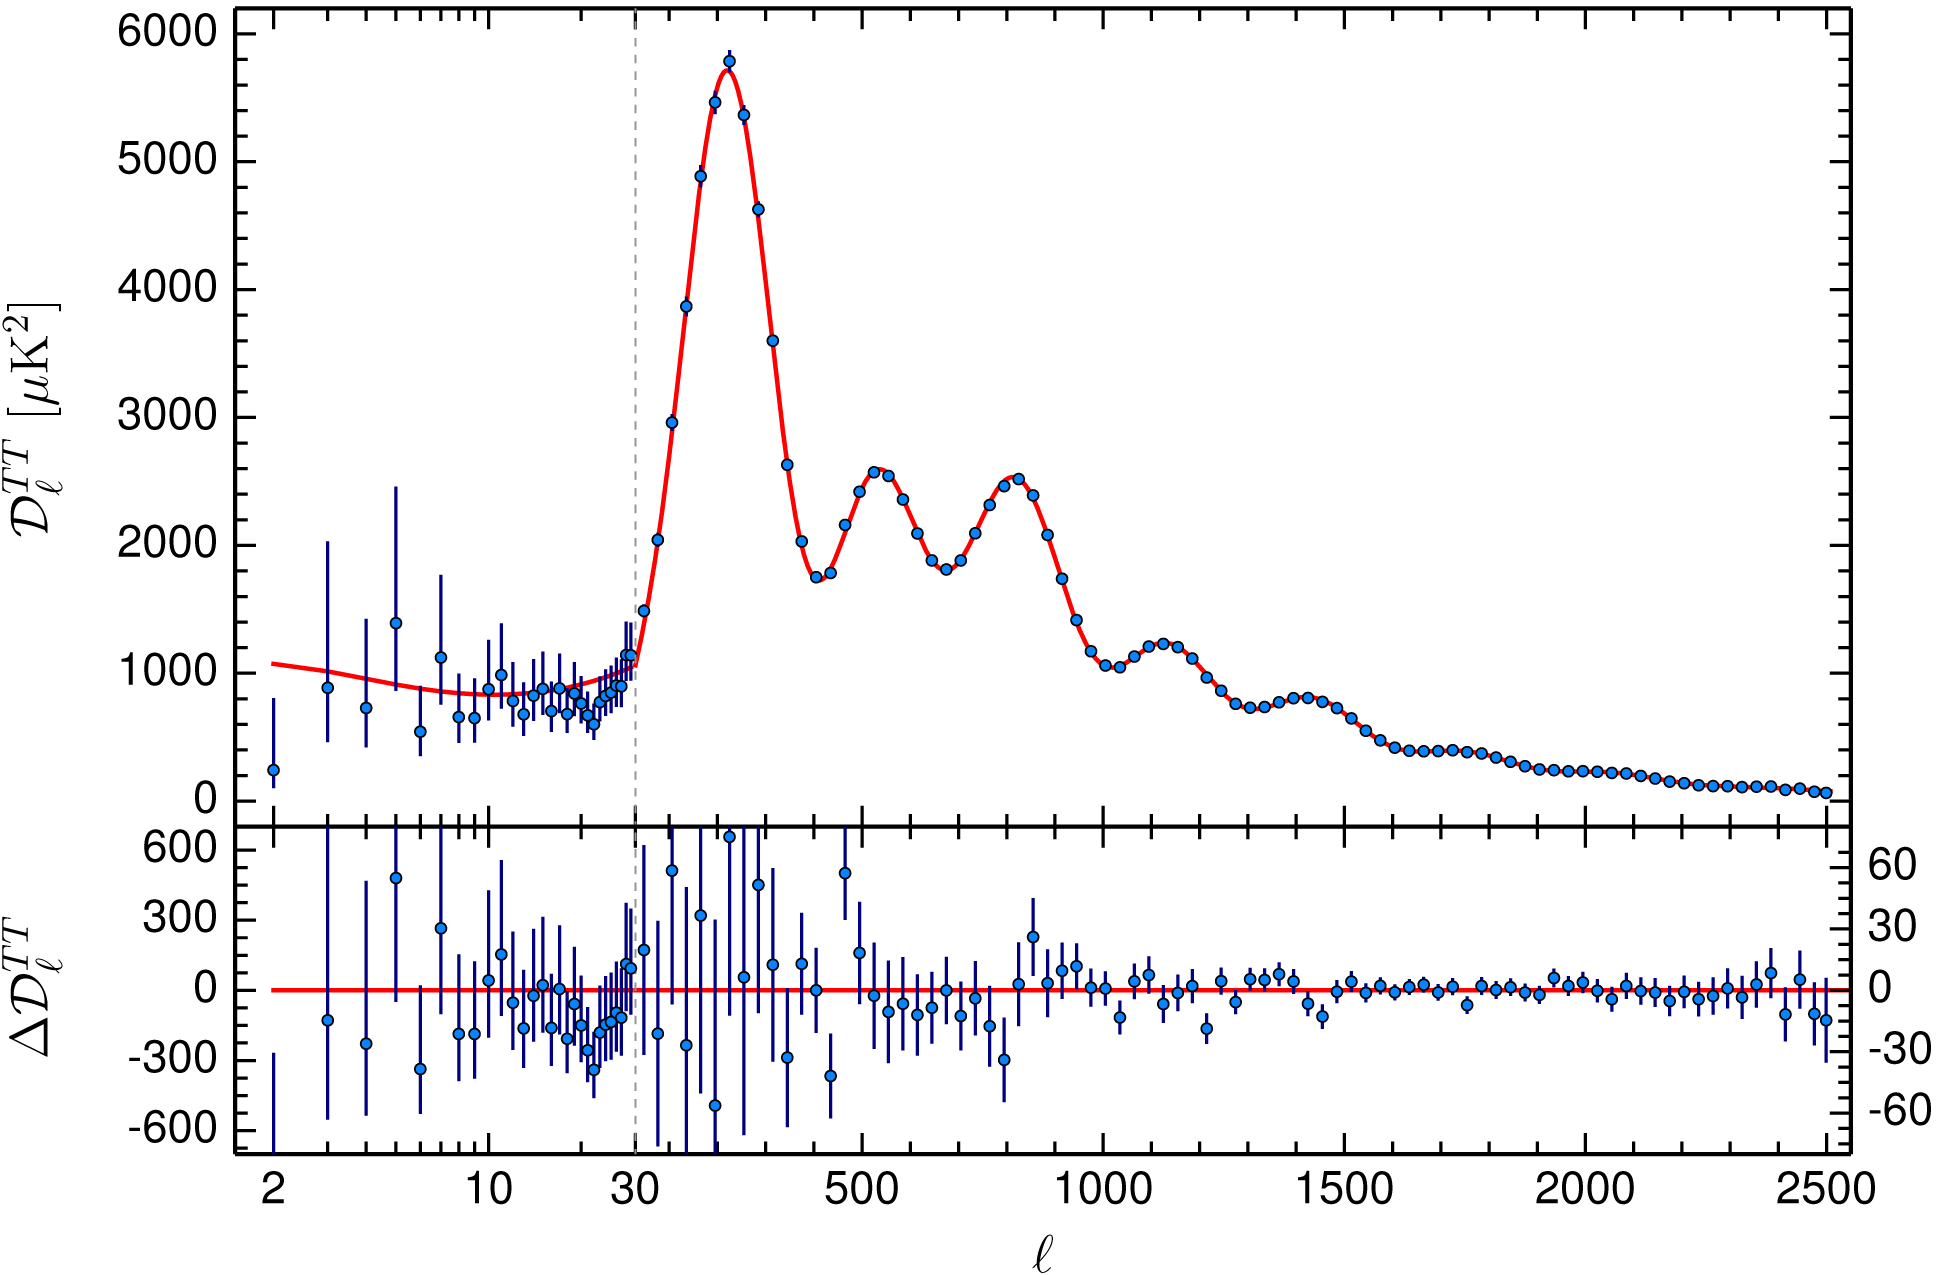
\includegraphics[width=\textwidth]{planck_aps}
        \caption{Plank angular power spectrum}
        \label{fig:planck_aps}
\end{figure}

For small values of $l$ we notice a plateu, caused by the Sachs-Wolfe
effect. At larger $l$, the spectrum exhibits a distinctive patterns of
patterns of peaaks and troughs, an evidence of acoustic oscillation in the
early Universe.

Data in the graph are well fitted by the standard
$\Lambda$CMD model. The main cosmological parameters defining this model of
the Universe are:

\begin{itemize}
        \item \textbf{Hubble constant:} it describes the expansion rate of
        the Universe at present time. The value obtained from Planck
        measures is

        \begin{equation}
                H_0 = \SI{67.8 \pm 0.9}{\kilo\meter\per\second\per\mega\parsec}.
        \end{equation}

        \item \textbf{Acoustic scale:} it is the characteristic angular
        scale of the fluctuations in CMB. This parameter is constrained by
        the position of the acoustic peaks. Plank observations yielded

        \begin{equation}
                \theta_* = \ang{0.59636 \pm 0.00025}.
        \end{equation}

        \item \textbf{Barionic matter density:} the matter density
        parameters can be extracted from the relative heights of the
        acoustic peaks. The value for baryons has been determined to be

        \begin{equation}
                \Omega_b h^2 = \num{0.02222 \pm 0.00023}
        \end{equation}

        where $h$ is defined by

        \begin{equation}
                H_0 \equiv \SI{100}{\hubble\kilo\meter\per\second\per\mega\parsec}
        \end{equation}

        \item \textbf{Dark matter density:} the value of the dark matter
        density parameter is

        \begin{equation}
                \Omega_c h^2 = \num{0.1197 \pm 0.0022}.
        \end{equation}

        \item \textbf{Dark energy density:} The value of the dark energy
        density parameter is estimed to be

        \begin{equation}
                \Omega_\Lambda = \num{0.685 \pm 0.012}.
        \end{equation}

        \item \textbf{Spectral index:} The inflationary paradigm predicts
        the power spectrum of primordial density perturbations to be a
        power law, $P\qty(\vb{k},t = t_\text{BigBang}) = k^n$. The index
        $n$, which is known as the spectral index, has the following value:

        \begin{equation}
                n = \num{0.9655 \pm 0.0062}.
        \end{equation}

        \item small-scale fluctuation in the CMB are damped by Thomson
        scattering from free electrons produced during rionization. Modes
        with wavelength smaller than the apparent horizon at reionization
        was suppressed by a factor $e^{-2\tau}$, where $\tau$ is the optical
        depth of Thomson scattering. The resulting value of $\tau$ from Placnk
        temperature power spectrum is

        \begin{equation}
                \tau = \num{0.078 \pm 0.019}.
        \end{equation}
\end{itemize}

\section{The Inflationary Paradigm}

The $\Lambda$CDM cosmological model describes very well some of the
cosmological observations, in particular the presence of the CMB black
body radiation and the abundance of light elements in the Universe.
Netherless, some fact about our universe linger unexplained.

\subsection{Open Issues of the Big Bang Cosmology}\label{ss:issues}

The three fundamental issue unsolved by the Big Bang model follow:

\begin{itemize}
        \item \textbf{Horizon problem:} observations of the cosmic
        microwave background radiation shows that our universe is very
        homogeneous and isotropic on the largest scales. In particular we
        know that zones of the Universe sitting at distance larger than the
        horizon during recombination and, for this reason, not causally
        connected, are characterized by the same CMB temperature.
        In fact, regions that in the standard Big Bang model would be causally
        connected at the time of the last scattering, subtend today an
        angle of \ang{\sim 1} in the sky.

        \item \textbf{Flatness problem:} current observations show a very
        flat universe, but the solutions of Friedmann equations for a
        radiation dominated universe describes flat curvature as a rather
        unstable condition. To explain the current spatially flat geometry
        we need to introduce ad hoc initial conditions in the model.

        \item \textbf{Initial conditions problem:} the Big Bang model
        does not furnish a physical mechanism to introduce density
        fluctuations in the early Universe. The presence of primordial
        fluctuations is required to explain the formation of galaxies and
        clusters we observe today.
\end{itemize}

\subsection{Inflation}

The issues presented in \autoref{ss:issues} can be solved introducing a
phase of accelerated expansion in the early universe, between
\SIlist{e-36;e-34}{\second} after the Big Bang. This idea is kwown as
\emph{inflation} or \emph{inflationary paradigm} and it was introduces by
Alan Guth in 1981.

\subsection{A Solution to Flatness and Horizon Problems}

To understand how inflation can solve the issues left unsolved by the Big Bang
model, we first define some useful quantities: the \emph{comoving particle
horizon} and the \emph{comoving apparent horizon}.

The comoving particle horizon is defined as

\begin{equation}
        \chi_H\qty(t) \equiv \int^t_0 \frac{c\dd{t'}}{a\qty(t')} =
        \int^a_0 \frac{\dd{a}}{a} \frac{c}{a\qty(t) H\qty(t)}
        \label{eq:horizons}
\end{equation}

and the quantity $d_{H,\text{co}}\qty(t) = \frac{c}{a\qty(t)H\qty(t)}$, which
appears in the second integral is the comoving apparent horizon.

If particles are separated by a comoving distance greater than
$\chi_H\qty(t)$ at a certain time $t$, they could not have been in causal
connection in the past. In turn, if the separating distance is more than
$d_{H,\text{co}}$, the two particles can not communicate \emph{now}. It is
possible that $\chi_H\qty(t)$ is much larger than $d_{H,\text{co}}$ now,
so that certain particles in the universe cannot communicate at present
time, but were in causal contact early on. We see from \autoref{eq:horizons}
that the condition for this to happen is a comoving apparent horizon much larger
in the early Universe than now. Hence a phase of decreasing comoving
apparent horizon is required.

A decreasing comoving apparent horizon means that scale of the CMB
radiation entering the horizon at present time were inside the comoving
apparent horizon during inflation (see \autoref{fig:horizon_inflation_solution}).
In other words, they are inside the comoving particle horizon. That is
enough to solve the horizon problem.

\begin{figure}
        \centering
        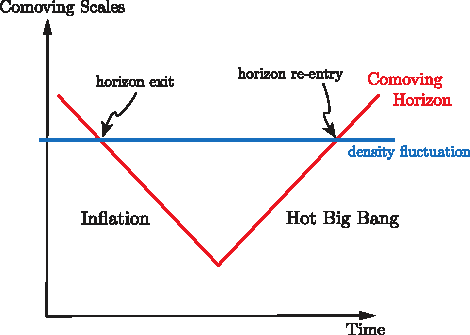
\includegraphics[width=\textwidth]{horizon_inflation_solution}
        \caption{Solution for the inflactionary problem (forse la prendo
        dalle dispense sull'inflazione)}
        \label{fig:horizon_inflation_solution}
\end{figure}


We can understand how the flatness problem is solved rewriting
\autoref{eq:friedmann_curvature} in term of the comoving apparent horizon
and taking its absolute value.  We obtain

\begin{equation}
        \abs{\Omega\qty(t) - 1} = k d_{H,\text{co}}.
\end{equation}

If the comoving apparent horizon decreases the Universe is driven toward
flatness. The solution $\Omega = 1$ is an attractor during inflation.

\subsection{Conditions for Inflation}

We have just seen that the a necessary condition for inflation is a
shrinking comoving apparent horizon in the early Universe. This is
equivalent to

\begin{equation}
        \dot d_{H,\text{co}} < 0.
\end{equation}

Calculation of the time derivative yields

\begin{equation}
        \frac{-\ddot a\qty(t)}{a^2\qty(t) H^2\qty(t)} < 0
\end{equation}

therefore a necessary condition for inflation is a phase of accelerated
expansion of the Universe,

\begin{equation}
        \ddot a\qty(t) > 0
\end{equation}

The second time derivative of the scale factor can be related to the first
time derivative of the Hubble parameter in this way

\begin{equation}
        \frac{\ddot a\qty(t)}{a\qty(t)} = H^2\qty(t)\qty(1 - \epsilon\qty(t)).
\end{equation}

$\epsilon$ is known as the \emph{slow-roll parameter} and is defined as
$\epsilon\qty(t) \equiv -\frac{\dot H\qty(t)}{H^2\qty(t)}$.
Therefore, for an accelerating phase to happen in the early universe is
required that

\begin{equation}
        \epsilon\qty(t) < 1.
\end{equation}

This condition implies that the fractional change of the Hubble parameter
is small during iflation. As a result we can assume

\begin{equation}
        H\qty(t) = H_I = \text{const.}
\end{equation}

during inflation.

Furthermore, looking at the second Friedmann equation, we infer that the condition $\ddot
a > 0$ requires

\begin{equation}
        P\qty(t) < -\frac{1}{3} \rho\qty(t).
\end{equation}

This demands the presence of a component of the cosmological fluid
characterized by the negative pressure, or, in an equivalent way, a
violation of the \emph{strong energy condition}.

\subsection{Physics of Inflation}

A simple physical model of inflation involves a single scalar field
$\phi\qty(\vb{\chi},t)$, known as \emph{inflaton}. The physical nature of
the inflaton is unknown, but we can simply use it as an \emph{order
paramerer} to parametrize the time-evolution of the inflationary energy
density.

The action associated to the a scalar field weakly coupled to gravity is

\begin{equation}
        S\qty[g,\phi] = S_{EH}\qty[g] + S_\phi\qty[g,\phi]
\end{equation}

where $S_{EH}\qty[g]$ is the gravitational Einstein-Hilbert action and
$S[g,\phi]$ is generic action for a scalar field. The explicit shapes of
these action action terms are

\begin{align}
        S_{EH}[g] & = \frac{1}{16\pi G} \int \sqrt{-g} R \dd[4]{\chi} \\
        S_\phi[g,\phi] & = \frac{\sqrt{-g}}{2}
        g^{\mu \nu}\partial_\mu\phi\partial_\nu\phi - V\qty(\phi)
\end{align}

where $V\qty(\phi)$ is a potential that describes the self-interactions of
the scalar field $\phi$.

The application of the variational principle to the action gives the
field equation of motion

\begin{equation}
        \frac{1}{\sqrt{-g}} \partial_\mu\qty(\sqrt{-g} \partial^\mu\phi) +
        V'\qty(\phi) = 0
\end{equation}

Assuming the FLRW metric for $g_{\mu \nu}$ and that we are working with an
homogeneous field $\phi\qty(\vb{\chi},t) \equiv \phi\qty(t)$, the equation
of motion become

\begin{equation}
        \ddot \phi + 3H \dot\phi + V'\qty(\phi) = 0
\end{equation}

the equation of motion of a damped harmonic oscillator and the field
evolves towards the minimum potential condition.

Under the same assumptions the energy momentum tensor of the field takes
the form of a perfect fluid, with the following pression and density,

\begin{align}
        \rho_\phi c^2 & = \frac{1}{2} \dot\phi^2 + V\qty(\phi) \\
        P_\phi & = \frac{1}{2}\dot\phi^2 - V\qty(\phi).
\end{align}

The usual $w$ proportionality parameter in the scalar field state equation
is

\begin{equation}
        w_\phi\qty(t) = \frac{\frac{1}{2} \dot\phi^2 - V\qty(\phi)}{\frac{1}{2}
        \dot\phi^2 + V\qty(\phi)}
\end{equation}

So in this case the slow-roll parameter becomes

\begin{equation}
        \epsilon\qty(t) \equiv \frac{3}{2} \qty(w_\phi\qty(t) + 1) =
        \frac{1}{2} \frac{\dot\phi^2\qty(t)}{H^2\qty(t)}
\end{equation}

Accelerated expansion takes place when $\epsilon\qty(t) < 1$. In particular
in the case limit defined by

\begin{equation}
        \dot\phi^2 \ll V\qty(\phi)
        \label{eq:sr_condition_1}
\end{equation}

$\epsilon\qty(t) \ll 1$, so as previuosly stated $H\qty(t) = H_I =
\text{const.}$ and we are in the de Sitter limit,

\begin{equation}
        P_\phi\qty(t) \approx -\rho_\phi\qty(t)
\end{equation}

that is, the inflaton behaves like a perfect fluid characterized by
negative pressure, as in the case of Dark Energy.

Accelerated expansion is sustained for a sufficiently long period of time
only if $\ddot \phi\qty(t)$ is small enough,

\begin{equation}
        \abs{\ddot\phi} \ll \abs{3H\dot\phi}, \abs{V'\qty(\phi)}.
        \label{eq:sr_condition_2}
\end{equation}

\autoref{eq:sr_condition_1} and \autoref{eq:sr_condition_2} are known as
\emph{slow-roll conditions}. Under them the equation of motion for the
scalar inflation field and the first Friedmann equation become

\begin{align}
        \dot\phi \approx & -\frac{V'\qty(\phi)}{3H}  \\
        H^2 \approx & \frac{8\pi G}{3} V\qty(\phi) = H_I
\end{align}

From the last equation we understand that during inflation the spacetime is
approximately de Sitter with the scale factor undergoing exponential growth,

\begin{equation}
        a\qty(t) \approx a\qty(t_I)e^{H_I\qty(t - t_I)}
\end{equation}

as expected. The inflation epoch comes to an end when thw slow-roll
conditions are violated,

\begin{equation}
        \epsilon(t_{I,\text{end}}) \equiv 1,
\end{equation}

from that time on the inflaction field kinetic energy starts to grow,
until the field potential comes to its minimun. The field energy is
dissipated in a process called \emph{reheating} and an epoch well
described by standard cosmology follows.

There are different inflaton potentials that guarantees slow-roll
conditions and each one of them corresponds to a distinc model of
inflation. An example of inflaton potential is shown in
\autoref{fig:inflaton_potential}.

\begin{figure}
        \centering
        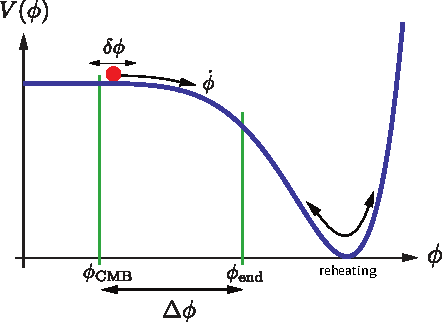
\includegraphics[width=\textwidth]{inflaton_potential}
        \caption{Example of inflaton potential}
        \label{fig:inflaton_potential}
\end{figure}

\subsection{Inflation and Primordial Perturbations}

The inflationary paradigm can also solve the initial conditions problem,
providing a physical mechanism to introduce perturbations in the early
universe. The non-uniformity arises from quantum fluctuations in the
inflaton field, which appear as linear perturbations of the field itself.

The Universe at the time of inflation was dominated by the inflation field,
therefore scalar, vector and tensor first order perturbations arised in
the spacetime metric. The three kind of perturbations evolve independently:
vector perturbations decay in an expanding universe. Instead, scalar and
tensor perturbations exihibit the following power spectra:

\begin{align}
        P_\phi & \\
        P_h & ,
\end{align}

respectively. The predicted values of the spectral
indeces are, $n_S \approx 1$ and $n_S \approx 0$.




\section{The CMB Polarization}

\chapter{LSPE/Strip}

\section{The LSPE Experiment}

\begin{figure}
        \centering
        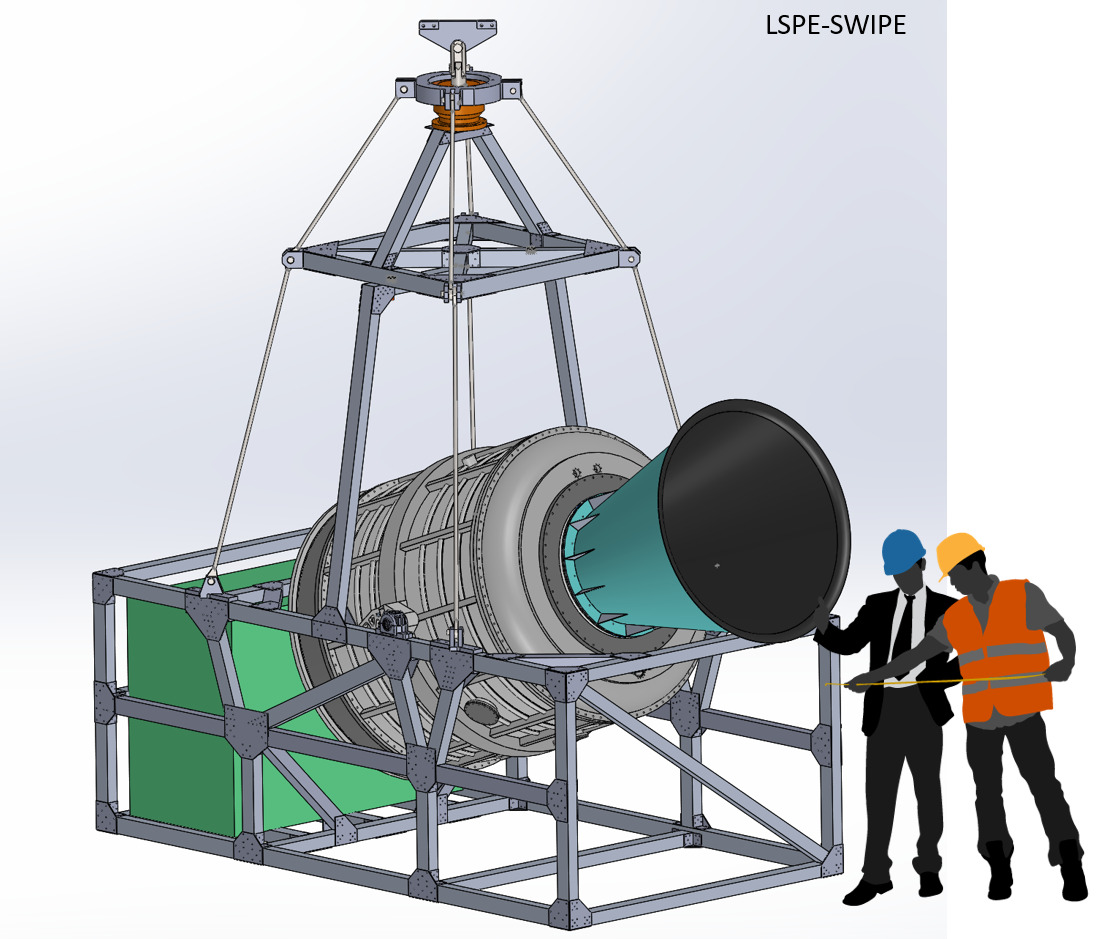
\includegraphics[width=\textwidth]{SWIPE}
        \caption{The SWIPE instrument}
        \label{fig:swipe}
\end{figure}

\section{The Strip Instrument}

\begin{figure}
        \centering
        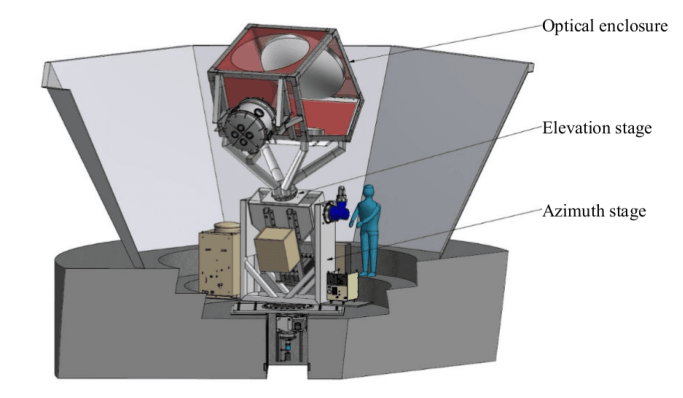
\includegraphics[width=\textwidth]{LSPE-Strip-optical-system}
        \caption{LSPE/Strip Optical System}
        \label{fig:lspe-strip_optical_system}
\end{figure}

\begin{figure}
        \centering
        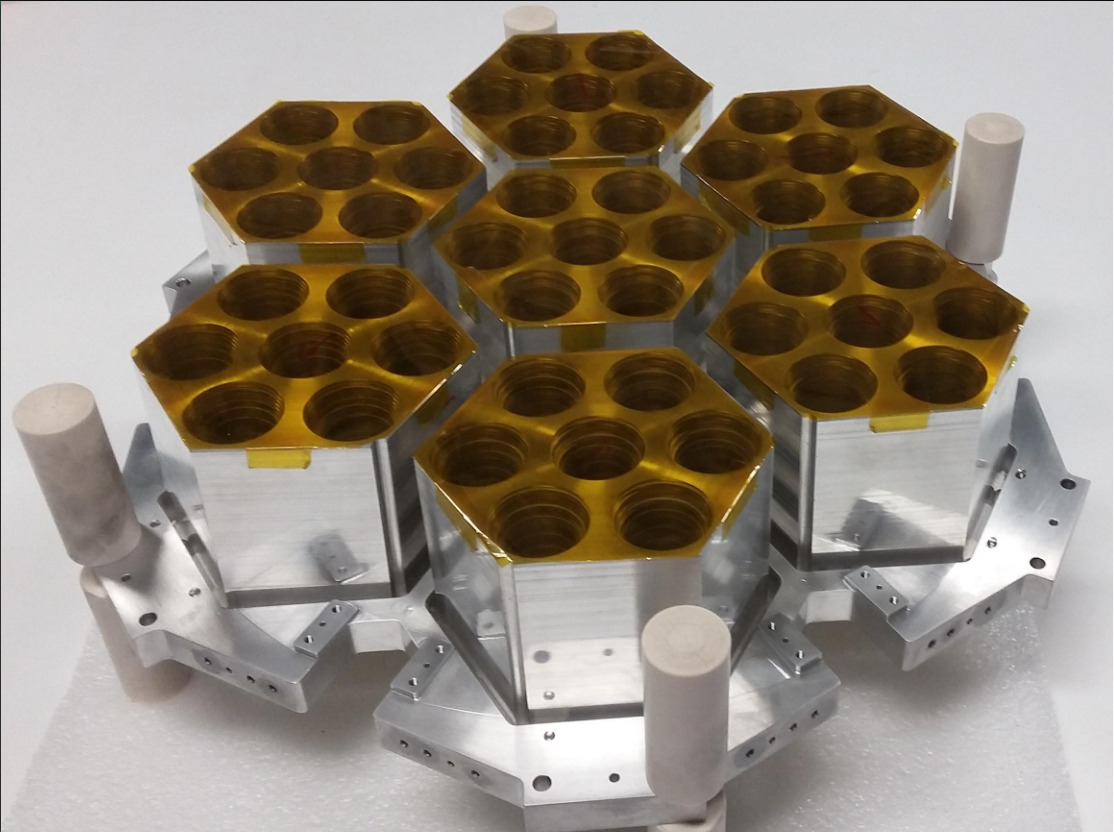
\includegraphics[width=\textwidth]{strip-focal-plane}
        \caption{Strip focal plane}
        \label{fig:strip_focal_plane}
\end{figure}

\subsection{The Observation Site}

The Strip instrument will be deployed to the \emph{Observatorio del Teide}
in the city of Iza\~na, in Tenerife Island, Spain (\ang{28;18;04} N,
\ang{16;30;38} W) (see \autoref{fig:observatorio_teide}). The astronomical
observatory is located on Mount Teide at \SI{2390}{\meter} above sea level
and it has been operated by the \emph{Instituto de Astrof\'isica de
Canarias} since 1964.

The Observatory's geographical location, combined with the excellent
quality of the sky for astronomy, led to Teide Observatory being dedicated
mainly to  the study of the sun. However, Teide Observatory hosted and
still hosts different CMB experiments.
The \emph{Tenerife Experiment} (1984) by Jodrell Bank (of the University of
manchester) was the first CMB experiment to be installed at the
observatory. It measured CMB temperature anisotropies on angular size of
\ang{5}. Currently the observatory hosts the \emph{Multi Frequency
Instrument} (MFI), the \emph{Thirty Gigahertz Instrument} (TGI) and the
\emph{Forty Gigahertz Instrument} (FGI) of the \emph{Q-U-I JOint TEnerife
CMB} (QUIJOTE-CMB) experiment by the Instituto de Astrof\'isica de
Canarias. QUIJOTE experiment aims to characterize the
polarization of the CMB radiation in the frequency range
\SIrange{10}{42}{\giga\hertz}. The Strip instrument will join the
international efforts to detect the B-modes of the CMB polarization,
observing the microwave sky from the same site.

The characteristic geographical and climatic non-homogeneity typical of
relatively small islands constitutes a challange for the estimate of the
systematics linked to atmospheric effects. This problem will be tackled in
the next chapters of this thesis.



\begin{figure}
        \centering
        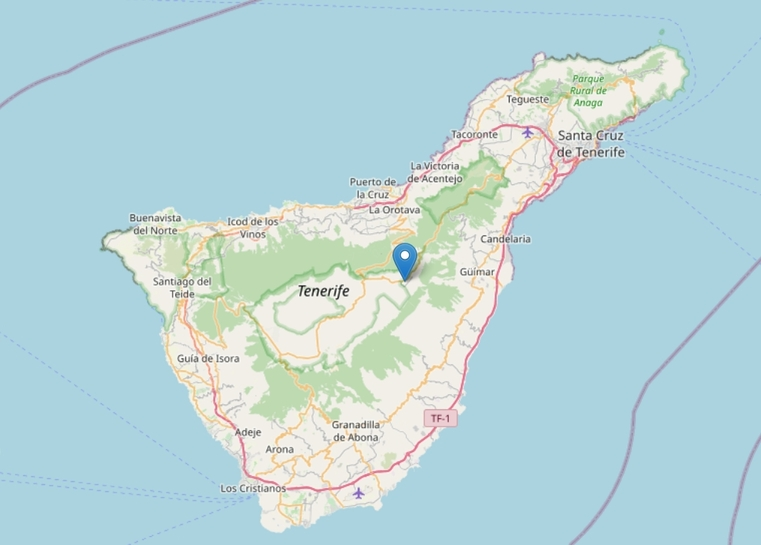
\includegraphics[width=\textwidth]{observatorio_teide}
        \caption{Observatorio del Teide}
        \label{fig:observatorio_teide}
\end{figure}


\chapter{The Atmospheric Emission Model}

Ground-based experiments have been playing and will continue to play a
prominent role in the observation of the cosmic microwave background
radiation temperature and polarisation anisotropies. As compared to
their space-borne or balloon-borne counterparts, ground-based experiments
can deploy larger primary reflectors, achieving higher angular resolution.
However, these instruments must deal with atmospheric effects.

The atmospheric radiation is almost unpolarized, therefore it does not
contribute directly to the signal acquired by instrumentation designed to
measure polarized sources, like the coherent polarimeters of the Strip
telescope. However, residual atmospheric emission inevitably increases the
optical power incident on the detectors and therefore their noise level. In
addition, temporal variations in emission, caused by variable water vapour
content, contribute low frequency correlated noise to the signal.

\section{Atmospheric Radiative Transfer}

The atmosphere can be viewed as a dielectric medium, whose effects on the
incoming electromagnetic radiation are charactherized by the complex permittivity

\begin{equation}
        \epsilon\qty(\nu) = \epsilon_r\qty(\nu) + i\epsilon_i\qty(\nu)
\end{equation}

where $\nu$ is the frequency of the incoming and radiation the real and
imaginary parts, $\epsilon_r$ and $\epsilon_i$ are linked by the
Kramers-Kronig relations

\begin{align}
        \epsilon_r\qty(s) & = \frac{1}{\pi}
        \principalvalue{\int^\infty_{-\infty}\dd{s'}
        \frac{\epsilon_i\qty(s)}{s' - s}} \label{eq:kk_relations_1} \\
        \epsilon_i\qty(s) & = -\frac{1}{\pi}
        \principalvalue{\int^\infty_{-\infty}\dd{s'}
        \frac{\epsilon_r\qty(s)}{s' - s}} \label{eq:kk_relations_2}.
\end{align}

The variable $s = \sigma + i 2\pi\nu$ is the complex frequency and $\sigma$
is the \emph{Neper frequency}.

As is shown in \autoref{fig:transmittance_teide}, contributions to the
atmospheric complex permittivity arise principally from
oxigen and water vapour molecules. Water vapour is responsible for most of
the continuum absorption in the \SIrange{400}{500}{\giga\hertz} frequency
range. The broad absorption oxigen band around \SI{60}{\giga\hertz} and the
oxigen line at \SI{119}{\giga\hertz} contribute to very strong absorption,
as the water vapour lines at \SIlist{22;183;325;380}{\giga\hertz} do. We will
show that the most problematic features of the atmospheric absorption spectrum
regarding the Q-band channels of the Strip telescope are in fact the
\SI{22}{\giga\hertz} water vapour line and the \SI{\sim 60}{\giga\hertz}
oxigen plateau.

\begin{figure}
        \centering
        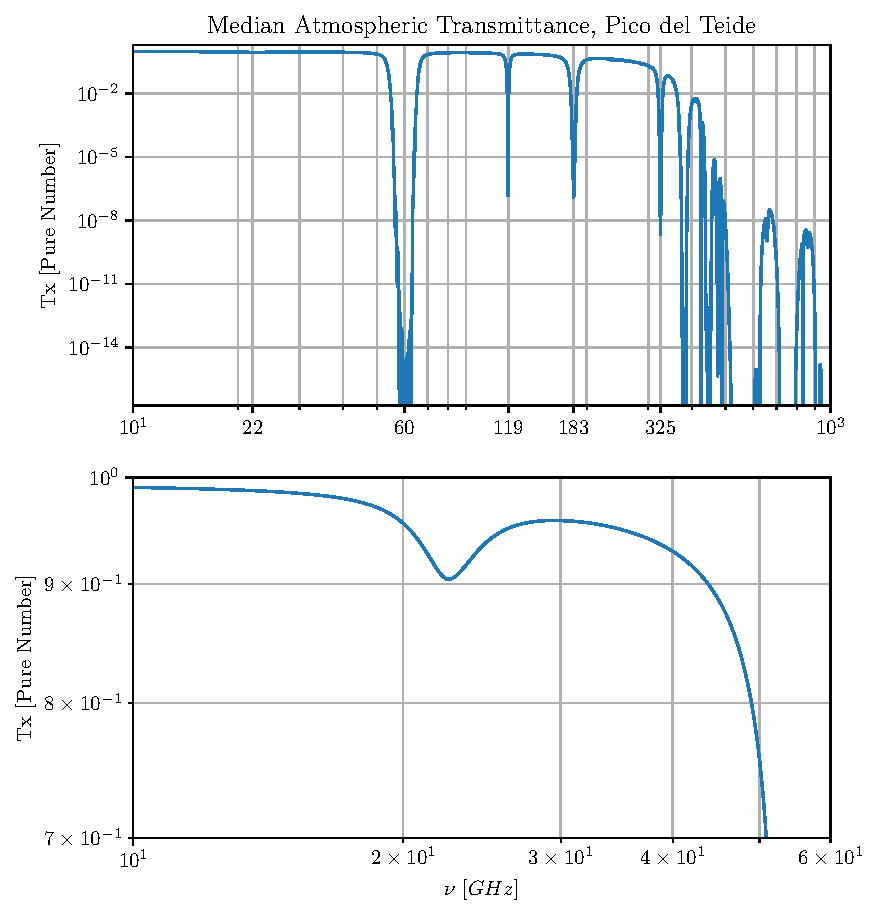
\includegraphics[width=\textwidth]{transmittance_Teide}
        \caption{Atmospheric transmittance at Pico del Teide and low
        frequencies detail. CAL software.}
        \label{fig:transmittance_teide}
\end{figure}


The real and imaginary parts of $\epsilon$ are related to the atmopshere
refractive index, $n\qty(\nu)$, and absorption coefficient, $\alpha\qty(\nu)$,

\begin{align}
        \epsilon_r\qty(\nu) & = \sqrt{n\qty(\nu)} \\
        \epsilon_i\qty(\nu) & = \frac{\lambda \alpha\qty(\nu)}{4\pi}
\end{align}

where $\lambda$ is the wavelength of the incoming radiation.

From \autoref{eq:kk_relations_1} and \autoref{eq:kk_relations_2} follows that
the refractive index and the absorption coefficient are note independent
quantities.

\subsection{Essential Quantities in Radiative Transfer Theory}

When the scale of a system greatly exceed the wavelength of propagating
radiation, we can consider radiation to travel in straight line, called
\emph{rays}. Starting from this observation we can devise a theory of
propagating rays, knwon as the \emph{radiative transfer theory}.

We consider an infinitesimal area $\dd{A}$ normal to the direction of a
specific ray and we take into account all the rays passing through $\dd{A}$
whose direction is whithin an infinitesimal solid angle $\dd{\Omega}$ of
the given ray (see \autoref{fig:rays_geometry}). The energy crossing
$\dd{A}$ in an infinitesimal time $\dd{t}$, in a frequency range $\dd{\nu}$
is

\begin{equation}
        \dd{E} \equiv
        I\qty(\vb{x},\Omega,\nu)\dd{A}dd{\Omega}\dd{\nu}\dd{t}
\end{equation}

which defines the \emph{specififc intensity}, $I\qty(\vb{x},\Omega,\nu) =
I_\nu$.

\begin{figure}
        \centering
        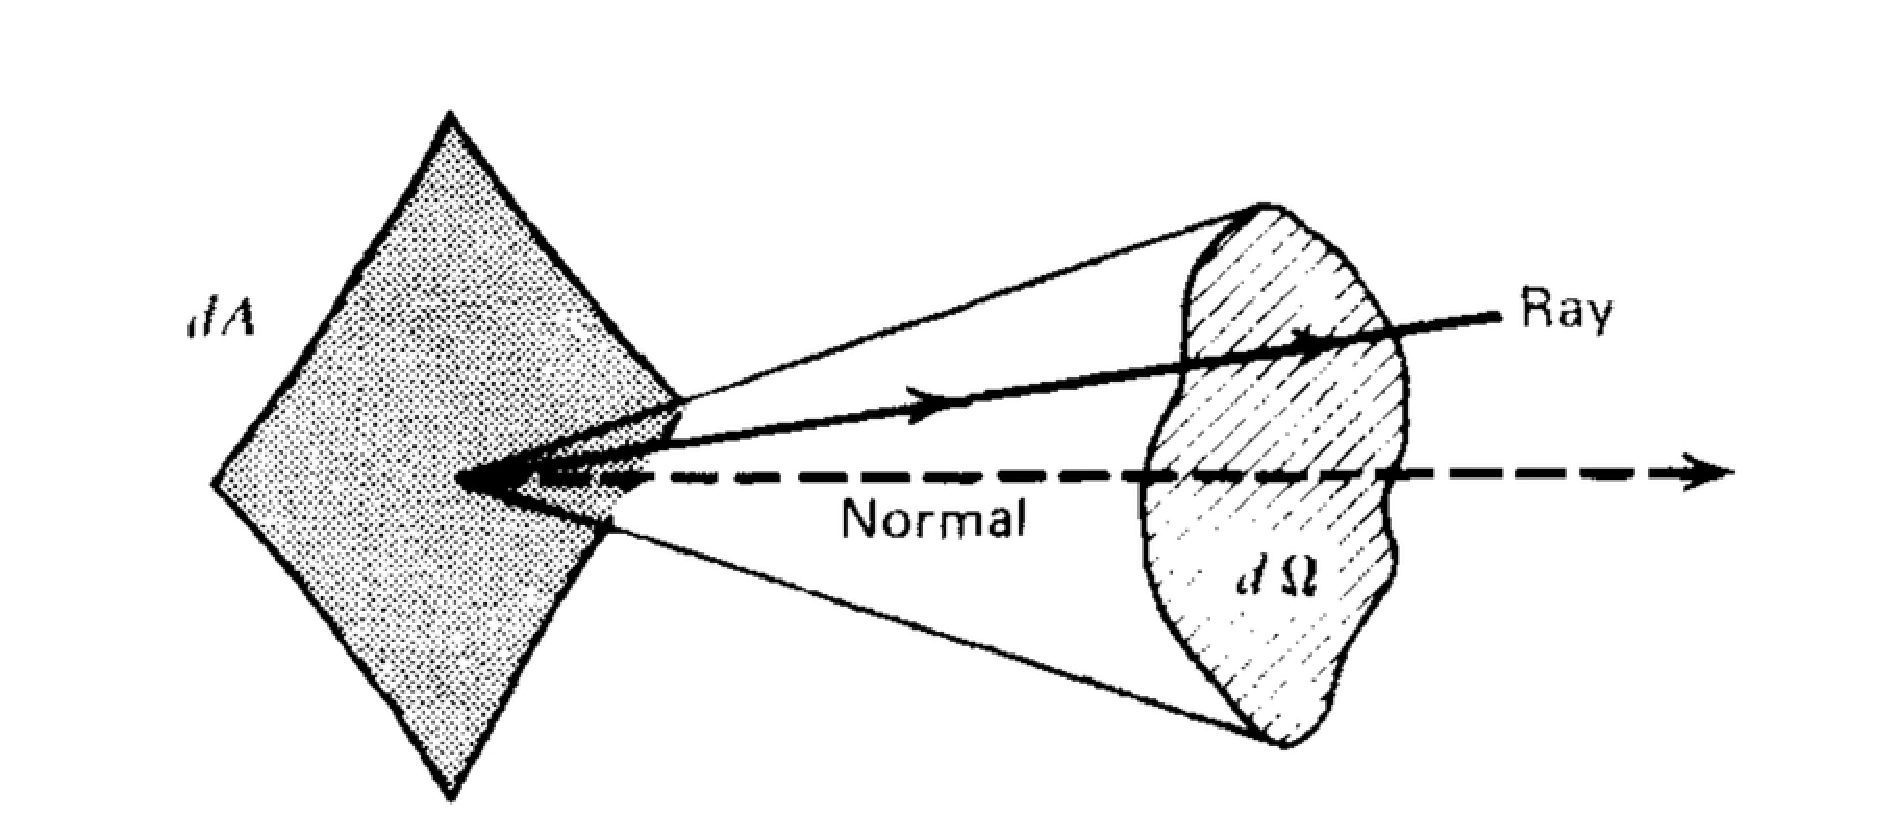
\includegraphics[width=\textwidth]{rays_geometry}
        \caption{Geometry for normally incident rays.}
        \label{fig:rays_geometry}
\end{figure}

The absorption coefficient $\alpha\qty(\nu) = \alpha_\nu$, introduced in the
previus section, represents the loss of intensity in a beam as it travels an
infinitesimal distance $\dd{r}$ in a dispersive medium. As the radiation
proceeds in the material, it runs into a random distribution of absorbers,
each presenting a cross section $\sigma_\nu$, of number density $n$. If we
assume that the mean interparticle distance is large in comparison to the
linear scale of the cross section, that is $n^{-\frac{1}{3}} \gg
\sqrt{\sigma_\nu}$, the total energy absorbed out of a beam passing
through a infinitesimal area $\dd{A}$ within a solid angle $\dd{\Omega}$ is

\begin{equation}
        \dd{E} = I_\nu \sigma_\nu n \dd{V} \dd{\Omega} \dd{\nu} \dd{t}
\end{equation}

where $\sigma_\nu n \dd{V} = \sigma_\nu n \dd{A} \dd{r}$ is the total
absorbing area presented by absorbers. The loss in energy, by definition,
can be expressed in terms of specifc brightness:

\begin{equation}
        \dd{E} = -\dd{I_\nu} \dd{A} \dd{\Omega} \dd{\nu} \dd{t}.
\end{equation}

Therefore if we combine the last two equations, we obtain

\begin{equation}
        \dv{I_\nu}{r} = -\sigma_\nu n I_\nu
        \label{eq:absorption}
\end{equation}

where $\sigma_\nu n = \alpha_\nu$. Note that absorption in
\autoref{eq:absorption} includes both \emph{true absorption} and
\emph{stimulated emission}, because both are proportional to the intensity
of the incoming radiation. Thus, $\alpha$ can be a positive or a negative
quantity.

The spontaneous emission, on the other hand, is independent of the
specific intensity of the beam. In the contest of radiative transfer theory
the quantity linked to this phenomenon is the \emph{spontaneous emission
coefficient} $j$, which is defined as the energy emitted
per unit time per unit solid angle and per unit volume:

\begin{equation}
        \dd{E} \equiv j\dd{V}\dd{\Omega}\dd{t}.
\end{equation}

A \emph{monochromatic spontaneous emission coefficient}, $j\qty(\nu) =
j_\nu$, can also be defined as

\begin{equation}
        j \equiv j_\nu \dd{\nu}.
\end{equation}

From now on we will refer to this quantity simply as the \emph{emission
coefficient}.
A beam of cross section $\dd{A}$, travelling an infinitesimal distance
$\dd{r}$, goes through a volume $\dd{V} = \dd{A} \dd{r}$. Therefore, from
the last two equations, we have

\begin{equation}
        \begin{split}
        \frac{\dd{E}}{\dd{A}\dd{\Omega}\dd{\nu}\dd{t}} & = j_\nu \dd{r} \\
        \dv{I_\nu}{r} & = j_\nu
        \label{eq:emission}
        \end{split}
\end{equation}

\subsection{The Radiative Transfer Equation}

The effects of emission and absorption can be incorporated into a sigle
equation giving the variation of specific intensity. From \autoref{eq:absorption}
and \autoref{eq:emission} we have

\begin{equation}
        \dv{I_\nu}{r} = -\alpha_\nu I_\nu + j_\nu
\end{equation}

which is known as the \emph{radiative transfer equation}. This equation
takes a particularly simple for if we realize the change of variable

\begin{equation}
        \begin{split}
                r \rightarrow \tau_\nu\qty(r) & \equiv \int^r_{r_0}
                \dd{r'}\alpha_\nu\qty(r') \\
                \dd{\tau_\nu} & = \alpha_\nu \dd{r}
        \end{split}
\end{equation}

where $\tau_\nu$ is known as the \emph{optical depth} or \emph{opacity}.
The transfer equation can now be divided by $\alpha_\nu$ and written as

\begin{equation}
        \dv{I_\nu\qty(\tau_\nu)}{\tau_\nu} = -I_\nu(\tau_\nu) +
        S_\nu\qty(\tau_\nu)
        \label{eq:radiative_transfer}
\end{equation}

where the function $S_\nu\qty(\tau_\nu)$ is known as the as the \emph{source
function} and is defined as

\begin{equation}
        S_\nu(\tau_\nu) \equiv
        \frac{j_\nu\qty(\tau_\nu)}{\alpha_\nu\qty(\tau_\nu)}.
\end{equation}

The source function and the opacity are convenient quantities in radiative
transfer theory, because they allow to reveal more clearly the intervals
along a ray that influence propagation of radiation the most.

\autoref{eq:radiative_transfer} can be now solved by regarding all
quantities as a function of the optical depth. First we multiply each side
of the equation by the positive quantity $e^{\tau_\nu}$:

\begin{equation}
        \dv{I_\nu\qty(\tau_\nu)}{\tau_\nu}e^{\tau_\nu} =
        -I_\nu\qty(\tau_\nu)e^{\tau_\nu} +
        S_\nu\qty(\tau_\nu)e^{\tau_\nu}
\end{equation}

then we integrate along a vertical path through the atmosphere:

\begin{equation}
        \begin{split}
                & \int^{\tau_{A,\nu}}_0 \dd{\tau_\nu}
                \dv{I_\nu\qty(\tau_\nu)}{\tau_\nu} e^{\tau_\nu} =
                -\int^{\tau_{A,\nu}}_0 \dd{\tau_\nu}
                I_\nu\qty(\tau_\nu) e^{\tau_\nu} +
                \int^{\tau_{A,\nu}}_0 \dd{\tau_\nu}
                S_\nu\qty(\tau_\nu) e^{\tau_\nu} \\
                & \eval{I_\nu\qty(\tau_\nu) e^\tau}^{\tau_{A,\nu}}_0
                -\int^{\tau_{A,\nu}}_0 \dd{\tau_\nu}
                I_\nu\qty(\tau_\nu) e^{\tau_\nu} = \\
                & = -\int^{\tau_{A,\nu}}_0 \dd{\tau_\nu}
                I_\nu\qty(\tau_\nu) e^{\tau_\nu} +
                \int^{\tau_{A,\nu}}_0 \dd{\tau_\nu}
                S_\nu\qty(\tau_\nu) e^{\tau_\nu} \\
                & I_\nu\qty(\tau_{A,\nu}) e^{\tau_{A,\nu}} -I_\nu\qty(0) =
                \int^{\tau_{A,\nu}}_0 \dd{\tau_\nu}
                S_\nu\qty(\tau_\nu) e^{\tau_\nu}
        \end{split}
\end{equation}

where integration by parts has been used in the right-hand side of the
equation and the quantity $\tau_{A,\nu}$ is the total opacity of the
traversed medium. If the last equation is divided by the positive factor
$e^{\tau_{A,\nu}}$ and terms are remanaged, the following equation is
obtained:

\begin{equation}
        I_\nu\qty(\tau_{A,\nu}) = I_\nu\qty(0) e^{-\tau_{A,\nu}} +
        \int^{\tau_{A,\nu}}_0 \dd{\tau_\nu}
        S_\nu\qty(\tau_\nu) e^{-\qty(\tau_{A,\nu} - \tau_\nu)}.
\end{equation}

This is known as the \emph{formal solution} of the radiative transfer
equation. The term $I_\nu\qty(0) e^{-\tau_{A,\nu}}$ represents the initial
intensity diminished by absorption and the second term in the sum stands
for the integrated source diminished by absorption.

\subsection{A Solution for Thermal Sources}

Thermal radiation is radiation emitted by matter in thermodynamic
equilibrium. When radiation is itself in thermodynamic equilibrium we
speak about \emph{black body radiation}, whose nature was already described
in \autoref{ss:cmb_bb}.

For black body radiation we have

\begin{equation}
        I_\nu \equiv B_\nu\qty(T_\text{phys})
\end{equation}

where $T_\text{phys}$ is the physical temperature of the radiation and of the
emitter and $B_\nu\qty(T_\text{phys})$ is the black body spectrum introduced
in \autoref{ss:cmb_bb},

\begin{equation}
        B_\nu\qty(T) = \frac{2h\nu^3}{c^2}
        \frac{1}{\exp(\frac{h\nu}{K_b T}) - 1}.
\end{equation}

This means that for black body radiation $I_\nu$ is an universal function
of $T$ and $\nu$, independent of the properties of the emitting body.

Kirchhoff's law states that the source function of a body in thermodynamic
equilibrium coincides with a black body spectrum

\begin{align}
        S_\nu & = B_\nu\qty(T_\text{phys}) \\
        j_\nu & = B_\nu\qty(T_\text{phys}) \alpha_\nu
\end{align}

where $T_\text{phys}$ is the physical temperature of the radiant body,
which from now on will be referred to simply as T.

The solution of the radiative transfer equation in the case of thermal
radiation is obtained from the formal solution by substitution of the
correct source function:

\begin{equation}
        I_\nu\qty(\tau_{A,\nu}) = I_\nu\qty(0) e^{-\tau_{A,\nu}} +
        \int^{\tau_{A,\nu}}_0 \dd{\tau_\nu} B_\nu\qty(T\qty(\tau_\nu))
        e^{-\qty(\tau_{A,\nu} - \tau_\nu)}.
        \label{eq:radiative_thermal}
\end{equation}

A further approximation can be made to simplify this result.
The exponential term in the Planck law can be expanded as

\begin{equation}
       \exp(\frac{h\nu}{K_b T}) = 1 + \frac{h\nu}{K_b T} + \order{\nu^2}.
\end{equation}

Therefore, for $\frac{h \nu}{K_b T}$, we obtain the \emph{Rayleigh-Jeans
approximation law}:

\begin{equation}
        B_\nu\qty(T) \approx \frac{2\nu^2}{c^2} K_b T.
\end{equation}

This relation is commonly used in astrophysics to characterize the
brightness of a radiation at a certain frequency. For any value value of
$I_\nu$ a corresponding \emph{brightness temperature} temperature can be
defined as

\begin{equation}
        I_\nu \equiv B_\nu\qty(T_b)
\end{equation}

or assuming that the Rayleigh-Jeans approximation is valid,

\begin{equation}
        T_b \equiv = \frac{c^2}{2\nu^2k} I_\nu.
\end{equation}

So, \autoref{eq:radiative_thermal} can be rewritten as

\begin{equation}
        T_b = T_b\qty(0) e^{-\tau_{A,\nu}} +
        \int^{\tau_{A,\nu}}_0 \dd{\tau_\nu} T\qty(\tau_\nu)
        e^{-\qty(\tau_{A,\nu} - \tau_\nu)}.
\end{equation}

The solution of this equation in the case of constant temperature along the
optical path, $T\qty(\tau_\nu) = T = \text{const.}$ is

\begin{equation}
        T_b = T_b\qty(0) e^{-\tau_{A,\nu}} + T\qty(1 -
        e^{-\tau_{A,\nu}}).
\end{equation}

If the opacity is large, the brightness temperature of the radiation
approaches the temperature of the medium.

\subsection{Local Thermodynamic Equilibrium}

It is possible to rewrite the radiative transfer equation in terms of
microscopic quantities. The theorical framework for the simple case of a
medium composed of emitters and absorbers characterized by two energy
levels was established by Einstein in
1917, in his famous article about the quantum theory of radiation.
The transfer equation in terms of Einstein coefficients reads

\begin{equation}
        \dv{I_\nu}{r} = -\frac{h\nu}{4\pi}\qty(n_1 B_{12} -
        n_2 B_{21})\phi\qty(\nu)I_\nu +
        \frac{h\nu}{4\pi} n_2 A_{21}\phi\qty(\nu)
\end{equation}

where

\begin{itemize}
        \item $n_1$ and $n_2$ are the number densities of atoms in energy
        levels 1 and 2, with $E_2 = E_1 + h\nu_0$;
        \item $B_{12}$ and $B_{21}$ are the Einstein absorption and
        stimulated emission coefficients, respectively;
        \item $A_{21}$ is the Einstein stimulated emission coefficient;
        \item and $\phi\qty(\nu)$ is the \emph{line profile function},
        which accounts for the fact that the energy difference $h\nu_0$i
        is not infinitely sharp. The line profile function is peaked at
        $\nu = \nu_0$ and is taken to be normalized:

        \begin{equation}
                \int^\infty_0 \phi\qty(\nu) = 1.
        \end{equation}

\end{itemize}

A comparison of this equation with \autoref{eq:radiative_transfer} allows
to obtain

\begin{align}
        \alpha_\nu & = \frac{h\nu}{4\pi}\qty(n_1 B_{12} -
        n_2 B_{21})\phi\qty(\nu) \\
        S_\nu & = \frac{n_2 A_{21}}{n_1 B_{12} - n_2 B_{21}}
\end{align}

which are the expressions for the absorption coefficient and the source
fuction in terms of microscopic quantities.

Using the Einstein \emph{detailed balance relations} for absorption and
emission

\begin{align}
        g_1 B_{12} & = g_2 B_{21} \\
        A_{21} & = \frac{2h\nu^3}{c^2} B_{21}
\end{align}

where $g_1$ and $g_2$ are statistical weights for energy level 1 and 2,
respectively, the absorption coefficient and the source function can be
rewritten as

\begin{align}
        \alpha_\nu & = \frac{h\nu}{4\pi} n_1 B_{12}
        \qty(1 - \frac{g_1 n_2}{g_2 n_1})\phi\qty(\nu)\\
        S_\nu & = \frac{2h\nu^3}{c^2}\qty(\frac{g_2 n_1}{g_1 n_2} - 1)^{-1}.
        \label{eq:gen_kirchhoff_law}
\end{align}

\autoref{eq:gen_kirchhoff_law} is known as the \emph{generalized Kirchhoff
law} and is valid even out of thermodinamic equilibrium. For a thermalized
system the number density for a certain energy level $i$, $n_i$, is
proportional to the \emph{Boltzmann dustribution} and to its degeneracy
number, $g_i$,

\begin{equation}
        n_i \propto \frac{g_i}{Q} \exp(-\frac{E_i}{K_b T})
\end{equation}

where

\begin{equation}
        Q \equiv \sum_j \exp(-\frac{E_j}{K_b T})
\end{equation}

is the \emph{canonical partition function}. The j index in the sum runs
over all states that are accessible to the to system. Therefore, in the
case of our two levels system we have that

\begin{equation}
        \frac{n_1}{n_2} = \frac{g_1 \exp(-\frac{E}{K_b T})}{
        g_2 \exp(-\frac{E + h\nu_0}{K_b T})} =
        \frac{g_1}{g_2} \exp(\frac{h\nu_0}{K_b T})
\end{equation}

and the expression for the absorption coefficient and the source function
become

\begin{align}
        \alpha_\nu & = \frac{h\nu}{4\pi} n_1 B_{12}
        \qty[1 - \exp(-\frac{h\nu}{K_b T})]\phi\qty(\nu)\\
        S_\nu & = \frac{2h\nu^3}{c^2}\qty[\exp(\frac{h\nu}{K_b T}) - 1]^{-1}
        = B_\nu\qty(T).
\end{align}

This thermal value for the source function is just a statement of the
Kirchhoff law. In this case matter is in thermal equilibrium with
itself but not necessarily with radiation, so it is said to be in \emph{local
thermodynamic equilibrium} (LTE). The atmosphere is in fact a dispersive
medium in local thermodinamic equilibrium: cosmic electromagnetic waves
such as solar radiation, the CMB, and radiations from the galaxy propagate
through it, but they are not in thermodinamic equilibrium with the medium.

Of course our atmosphere is not an ensamble of two levels emitters and
absorbers, like the one we have presented above. Instead, it is in local
thermodinamic equilibrium in a classical sense: the local distribution of
particle velocities within it corresponds to the \emph{Maxwell-Boltzmann}
distribution,

\begin{equation}
        p\qty(v) = \qty(\frac{m_*}{2\pi K_b T})^{3/2}
        \exp(-\frac{m_* v^2}{2 K_b T})
\end{equation}

where $m_*$ is a reference mass for particles in the atmosphere.
This means that in principle we can split the atmosphere in an arbitrary
number of vertical layers, assuming the thermodynamic temperature is
constant within each one.  The radiative transfer equation can then be
written down and solved for every layer and the solutions connected. This
constitutes a simplified view of the numerical approach we have adopted in
the context of this thesis to obtain estimates for atmospheric brightness
temperatures.

\section{Atmospheric Spatial Structures}

\chapter{The Atmospheric Statistical Picture}\label{ch:statistical_picture}

In this chapter a method to build a \emph{statistical picture} of the
atmosphere is presented. First the ERA5 dataset is introduced: this
constitutes the set of statistical populations for the relevant meteorological
parameters that we have choosen to achieve this result; then the statistical
picture of the atmosphere is defined and the described in details; finally,
the mathematical objects we have used to describe expected daily and annual
variations of meteorological parameters at Pico del Teide are analyzed.

These results form the basis to get an estimate of the atmosphere
brightness temperature in the microwave range. This contribution, and its
seasonal variations as well, will be studied in the following chapters.

\section{The ERA5 Dataset}

As we have discussed in \autoref{ch:atm_model}, to calculate the extra load
caused by atmospheric effects, we must solve the radiative transfer equation
in the case of a dispersive medium at local thermodynamic equilibrium. The
solution depends on the physical properties of the medium. In particular,
it is determined by its physical temperature, $T$, and absorption
coefficient, $\alpha_\nu$. In turn, these quantities depends on a set a
meteorological parameters, which undergo seasonal variations.

In order to create a reliable statistical representation of these daily and
annual variations, we employed the ERA-5 dataset by the \emph{European
Centre for Medium-Range Weather Forecasts} (ECMWF). ECMWF uses forecast
models and data assimilation systems to \emph{reanalyse} archived
meteorological observations, creating global datasets describing the
recent history of the atmosphere, land surface, and oceans. In particular,
ERA5 provides hourly estimates of a large number of atmospheric, land and
oceanic climate variables. The data cover the whole Earth surface and
resolve the atmosphere using \num{137} levels from the surface up to a
height of \SI{80}{\kilo\meter}. ERA5 reanalysis relies on the \emph{Global
Circulation Model} (GCM) algorithm (McGuffie, Henderson-Sellers) making use
of the historical measures as forcing terms into GCM simulations to produce
data homogeneously gridded characterized by high spatial and temporal
resolution.

\autoref{fig:pwv_canary_islands} shows PWV distribution from ERA5 dataset
in Canary Island for the twelfth hour of the first day of the 1980. The
archipelago in covered by a grid of \num{30} by \num{30} \si{\kilo\meter}
\emph{pixels}  (\ang{0.25} by \ang{0.25} in geographic coordinate system).
As expected, precipitable water vapour takes its lowest values for
continental lands, its greatest values for pixels covering ocean and
intermediate values in correspondence of islands. \autoref{fig:pwv_tenerife}
focuses on Tenerife islands, showing that the whole site is covered by only four
pixels, which are delimited by a fuchsia perimeter in the figure.
In the following chapters we will prove that ERA5 spatial
resolution is in fact not enough to describe the specific meteorological
conditions at Pico del Teide, and at observation sites found on
small islands in general.

\begin{figure}
        \centering
        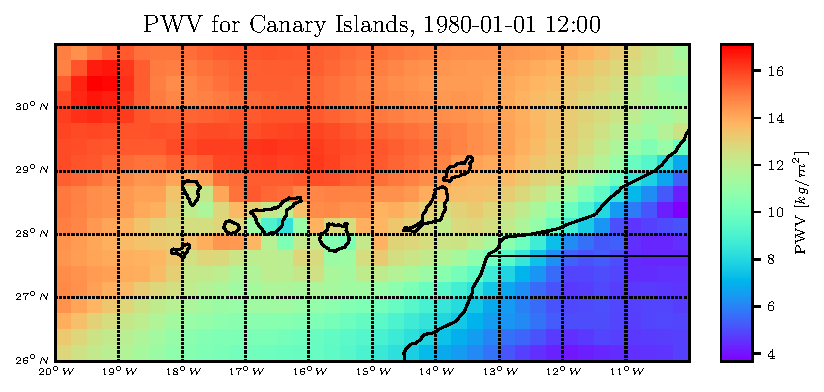
\includegraphics[width=\textwidth]{PWV_Canary_Islands_1980-01-01_12-00}
        \caption{PWV Canary Islands}
        \label{fig:pwv_canary_islands}
\end{figure}

\begin{figure}
        \centering
        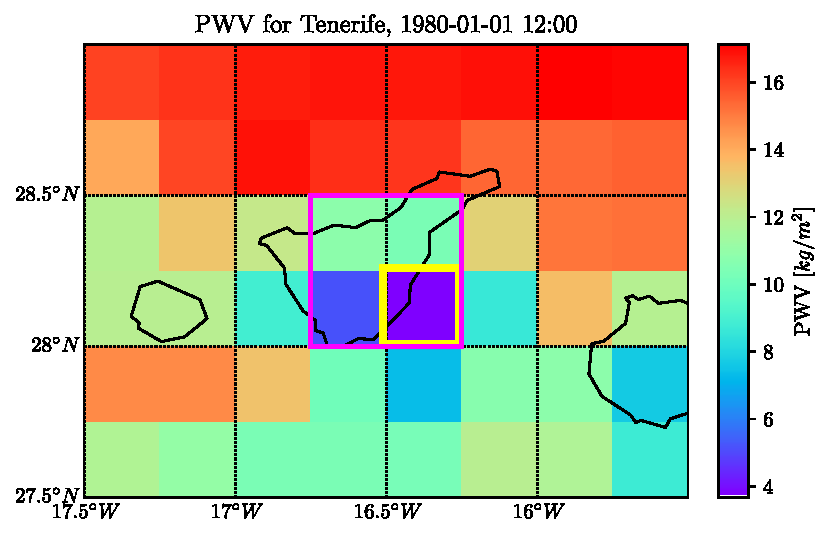
\includegraphics[width=\textwidth]{PWV_Tenerife_1980-01-01_12-00}
        \caption{PWV Tenerife}
        \label{fig:pwv_tenerife}
\end{figure}

\subsection{The Set of Relevant Meteorological Parameters}

Climate reanalysis data ranging from January the 1th 1979 to November
the 21th 2020 have been acquired by means of the ECMWF Web API, for a total of
\num{367200} hours in UTC. Downloaded data concern only one of the pixels found in
\autoref{fig:pwv_tenerife}: the one including the territory of Teide
observatory, which in the figure is enclosed by a yellow
square.

The relevant parameters, essential to provide a complete description of our
atmosphere, have been selected, for a total of seven quantities:

\begin{itemize}
        \item \textbf{total column cloud liquid water} (\textbf{tclw}):

        the amount of liquid water contained within cloud
        droplets in a column extending from the surface of the Earth to the
        top of the atmosphere, measure in \si{\kilo\gram\per\square\meter}.
        Rain water droplets, which are much larger
        in size (and mass), are not included in this parameter;

        \item \textbf{total column cloud ice water} (\textbf{tciw}):

        the amount of ice contained within clouds in a column extending
        from the surface of the Earth to the top of the atmosphere,
        measured in \si{\kilo\gram\per\square\meter}. Snow
        (aggregated ice crystals) is not included in this parameter;

        \item \textbf{total column water vapour} (\textbf{tcwv}) or \textbf{precipitable
        water vapour} (\textbf{PWV}):

        the total amount of water vapour in a column
        extending from the surface of the Earth to the top of the
        atmosphere, measured in \si{\kilo\gram\per\square\meter};

        \item \textbf{skin temperature} (\textbf{skt}):

        the temperature of the surface of the Earth, measured in
        \si{\kelvin};

        \item \textbf{surface pressure} (\textbf{sp}):

        the pressure of the atmosphere on the surface of land, sea and
        in-land water, measured in \si{\pascal};

        \item \textbf{10 meter temperature} (\textbf{T10M}):

        this parameter is not present in the ERA5 database, then it has
        been deduced from the \emph{2 meter temperature} (2t) parameter
        assuming a linear decrease in troposphere temperature of
        \SI{6.5e-3}{\kelvin\per\meter}. The 2t parameter represents the
        temperature of air at \SI{2}{\meter} above the surface of land, sea
        or in-land waters;

        \item \textbf{10 meter V wind component} (\textbf{10v}):

        the northward component of the 10m wind. It is the horizontal speed
        of air moving towards the north, at a height of ten meters above
        the surface of the Earth, measured in \si{\meter\per\second};

        \item \textbf{10 meter U wind component} (\textbf{10u}):

        like the latter parameter, but for the eastward component of the
        wind speed.
\end{itemize}

The totality of these meteorological parameters is necessary to describe
atmospheric radiative contribution and spatial structures. However, the
skin temperature ($T_s$), the surface pressure ($P_s)$ and the precipitable
water vapour (PWV) are enough to provide a first estimate of the extra
white noise load on detectors.

\begin{figure}
        \centering
        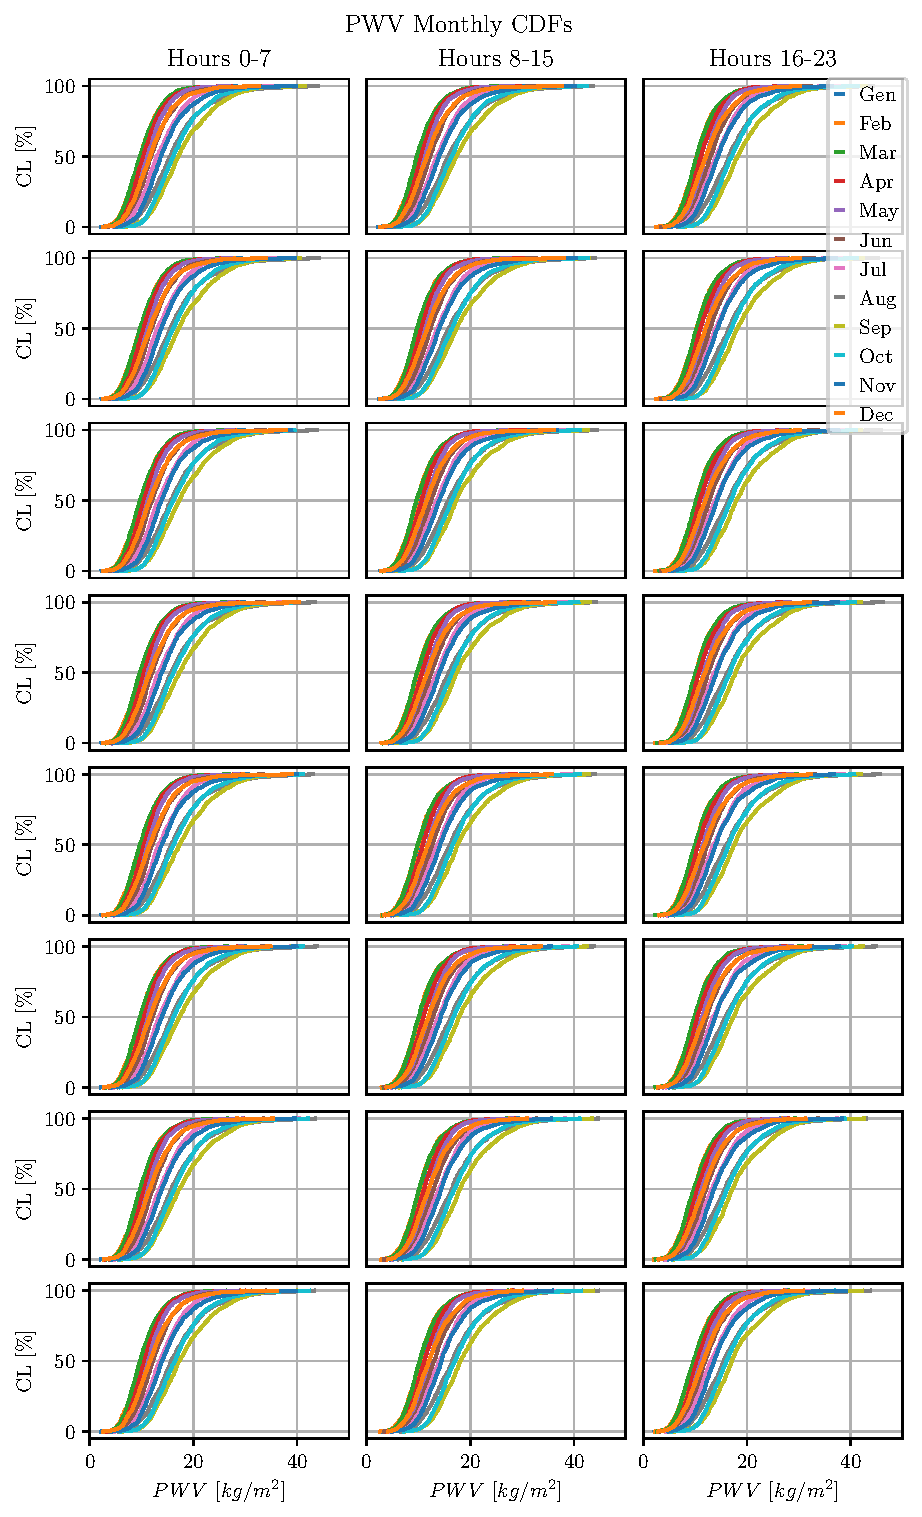
\includegraphics[width=0.83\textwidth]{PWV_Monthly_CDFs}
        \caption{PWV Monthly CDFs}
        \label{fig:pwv_monthly_cdfs}
\end{figure}

\section{The Seasonal Matrices}

\begin{figure}
        \centering
        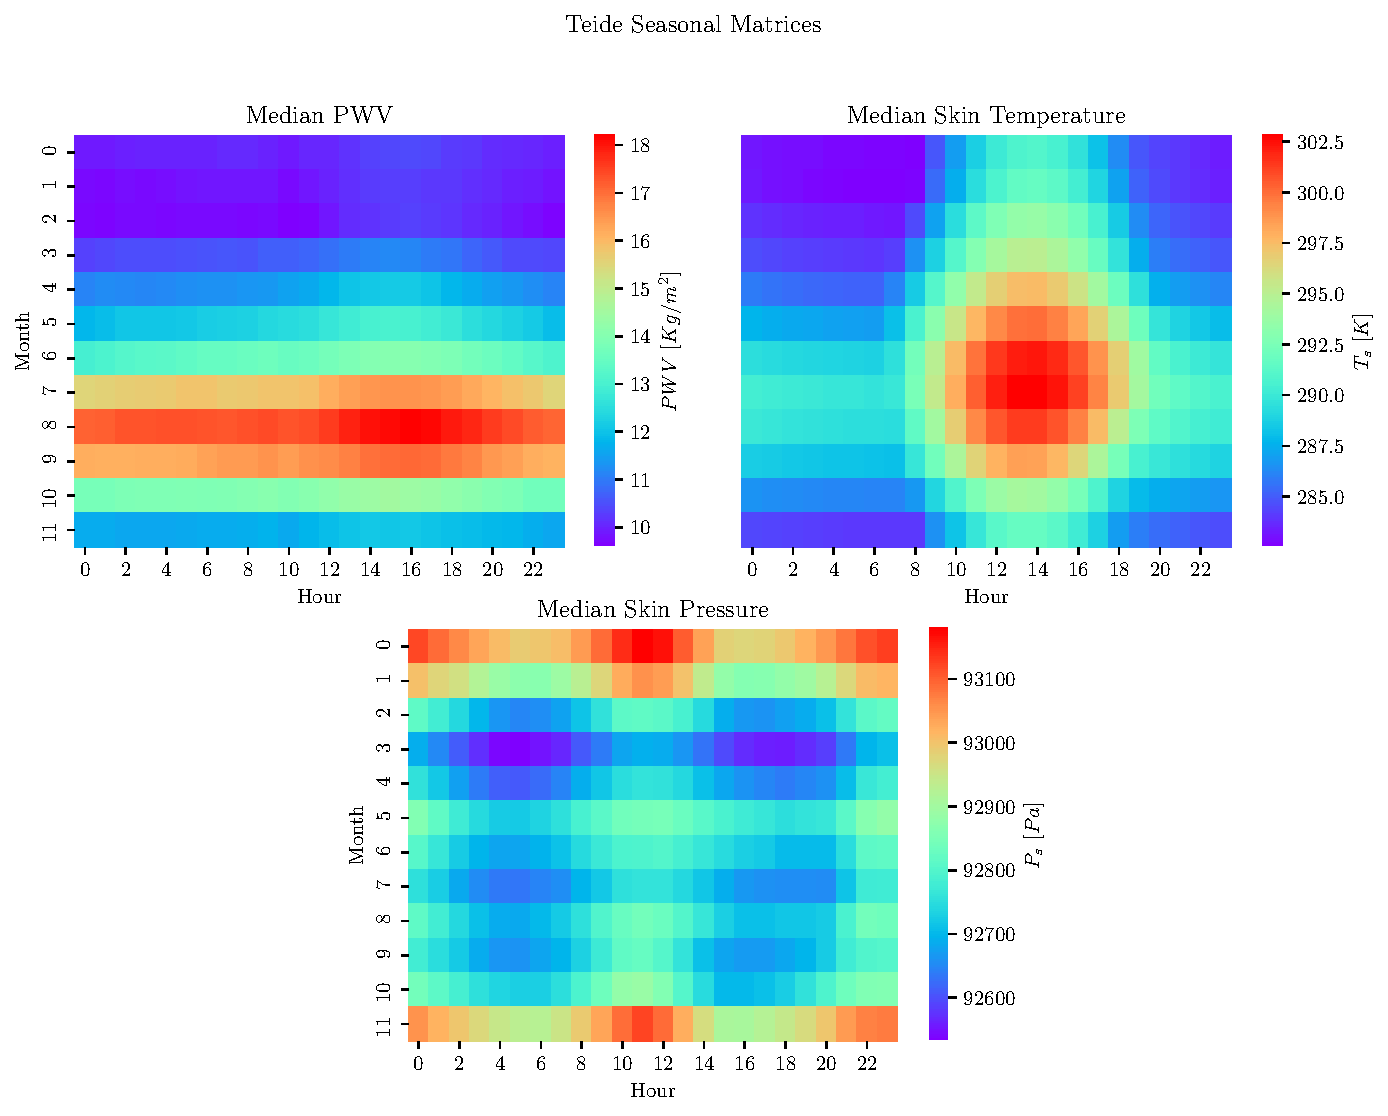
\includegraphics[width=\textwidth]{Teide_Seasonal_Matrices}
        \caption{Pico del Teide Seasonal Matrices}
        \label{fig:teide_seasonal_matrices}
\end{figure}


\chapter{Atmospheric Temperatures Variations}\label{ch:atm_variations}

In the current chapter we present the numerical methods and tools
implemented to estimate atmospsheric brighness temperatures at our
observation site. We introduce the CMB Atmospheric Library first. This is
the software library that has been employed to perform montecarlo
simulations of the meteorological parameters and to solve the radiative
transfer equation. Then, we present and discuss our numerical results: the
seasonal matrices of atmospheric brightness temperatures.

\section{The CMB Atmospheric Library}

The \emph{CMB Atmospheric Library}
(CAL)\footnote{\url{https://github.com/cmbgroundbased/cal}} is a free and
open source software library that has been developed to produce computer
simulations of atmospheric effects and telescope observations for
ground-based CMB experiments. CAL incorporates code extracted from the
well-known \emph{Time Ordered Astrophysics Scalable Tools} (TOAST) software
framework, making it and independent module, which can be exploited by
different CMB ground-based experiments. The CMB Atmospheric Library core is
written in \texttt{C++} programming language, in order to maintain high
performance.  However, \texttt{Python} programming language bindings are
provided to simplify its integration in \texttt{Python} based simulation
pipelines.

CAL can be used to solve the atmospheric radiative transfer equation
(discussed in \autoref{ss:radiative_transfer_eq}). To this end, the library
ships with
\emph{libaatm}\footnote{\url{https://github.com/hpc4cmb/libaatm}}, a
repackaged version of the \emph{Alma Atmospheric Transmission at Microwaves
Tools} (cit pardo), a model of the longwave atmospheric spectrum based on
broadband measurements and calculations. The model is fully applicable from
\SIrange{0}{2}{\tera\hertz} while including lines up to
\SI{10}{\tera\hertz}. Its primary goal is to simulate the millimeter and
submillimeter regions accessible from the ground.  libaatm discretizes the
atmosphere in a finite number of vertical layers, from sea level to the
tropopause, by a predefined internal profile. Then, the radiative transfer
equation is solved for each layer and the obtained solutions are connected,
by requiring continuity conditions to be satisfied at the boundaries
between different layers.

\subsection{CAL Relevant Methods}

Here we describe the relevant methods which are provided by CAL and we have
used in this work:

\begin{itemize}
        \item \texttt{Weather}:

        This class can be initialized with the CDFs \texttt{.fits} file,
        described in \autoref{s:CDF_fits_file}. It takes in input
        an UTC time structure with time resolution of \num{1} hour and
        returns pseudo-random realizations of meteorological parameters,
        determined by the probability distributions derived from the input
        \texttt{.fits} file.

        \item \texttt{atm\_atmospheric\_loading}:

        A wrapper function around libaatm methods. It solves the radiative
        transfer equation for a realization of the atmosphere defined by
        the values of $T_s$,
        $P_s$ and PWV, which are expected as input. It returns the value of sky
        brightness temperature in \si{\kelvin} (Rayleigh-Jeans) at a given
        frequency value, specified in input.

        \item \texttt{atm\_absorption\_coefficient}:

        As the latter, this function solves the radiative transfer equation,
        but it returns the total absorption coefficient,

        \begin{equation}
                \alpha_A\qty(\nu) = 1 - e^{-\tau_A\qty(\nu)}
        \end{equation}

        for the specified atmosphere realization at a given frequency.
\end{itemize}

These three objects hide a significant implementation complexity, but are
simple in use. They can be jointly used to produce Monte Carlo simulations of
atmospheric brightness temperature at Pico del Teide, or at any other site
of interest.

%\section{The \texttt{tatmget} Computer Program}

\section{Atmospheric Temperatures Seasonal Matrices}

Atmospheric brightness temperatures can be computed starting from the
methods provided by the CMB Atmospheric Library, by making use of
\autoref{eq:rte_solution_thermal}:

\begin{equation}
        T\qty(1 - e^{-\tau_{A,\nu}})= T_b - T_b\qty(0) e^{-\tau_{A,\nu}}.
\end{equation}

The terms in the equation have been rearranged, because right now we are
not interested in the total sky brightness temperature, $T_b \equiv
T_\text{sky}$, but only in the contribution due to the atmosphere, $T\qty(1
- e^{-\tau_{A,\nu}}) \equiv T_\text{atm}$, which depends on atmospheric
physical properties. $T_b(0)$ is the brightness temperature of the incoming
cosmic radiations. If it is assumed that the instrument is observing a
relatively clear patch of sky this contribution is dominated by the cosmic
microwave background radiation. Therefore, we have:

\begin{equation}
        T_\text{atm}\qty(\nu) = T_\text{sky}\qty(\nu) -
        T_\text{CMB}\qty(\nu)e^{-\tau_A\qty(\nu)}
        \label{eq:tatm_formula}
\end{equation}

where $T_\text{CMB}\qty(\nu)$ is the CMB brightness temperature expressed
in \si{\kelvin} Rayleigh-Jeans and $\tau_A\qty(\nu)$ is the total optical
depth of the atmosphere. $T_\text{CMB}\qty(\nu)$ is diminished by an
exponential factor that depends on the total opacity.

$T_\text{sky}\qty(\nu)$ and $\tau_A\qty(\nu)$ can be computed for arbitrary
frequencies and atmosphere realizations by means of the three CAL methods
listed above. The value of $T_\text{CMB}$ has been measured with great
precision and can be easily converted in \si{\kelvin} Rayleigh-Jeans for any
given frequency.

A population of \num{1000} values of $T_\text{atm}$ at \SI{43}{\giga\hertz}
(Strip Q-band central frequency) has been computed for every hour of each
typical day of every month of the year, for a total of \num{288}
statistical populations. The \texttt{Weather} class has been initialized
with the CDFs \texttt{.fits} file, which in turn was obtained starting from
the ERA5 meteorological data for Pico del Teide. Then, each statistical
population has been subdivided into \num{10} samples of \num{100} elements
each. Expectation values for each population has been computed, using mean
and median as estimators. The corresponding standard errors have been
obtained by calculation of standard deviation of the mean, in the case of
the first estimator, and making use of a bootstrapping technique, from the
samples, in the case of the second one.

Our results are shown in \autoref{fig:tatm_nocal} and
\autoref{fig:tatm_matrices_nocal}. Median daily variations in the
atmosphere brightness temperature for each month of the year are shown in
\autoref{fig:tatm_nocal}. The corresponding seasonal matrices, showing mean
and median seasonal variations in $T_\text{atm}$, are represented in
\autoref{fig:tatm_nocal}.

The annual average brightness temperature daily excursion is \SI{0.69 \pm
0.06}{\kelvin}, a small value if compared to the average annual
excursion: \SI{3.67 \pm 0.08}{\kelvin}. In particular
September, October and November are charactherized by larger values of
atmospheric brightness temperature, suggesting that bad weather days are more
frequent during these months, making them less suitable for observations.

\begin{figure}
        \centering
        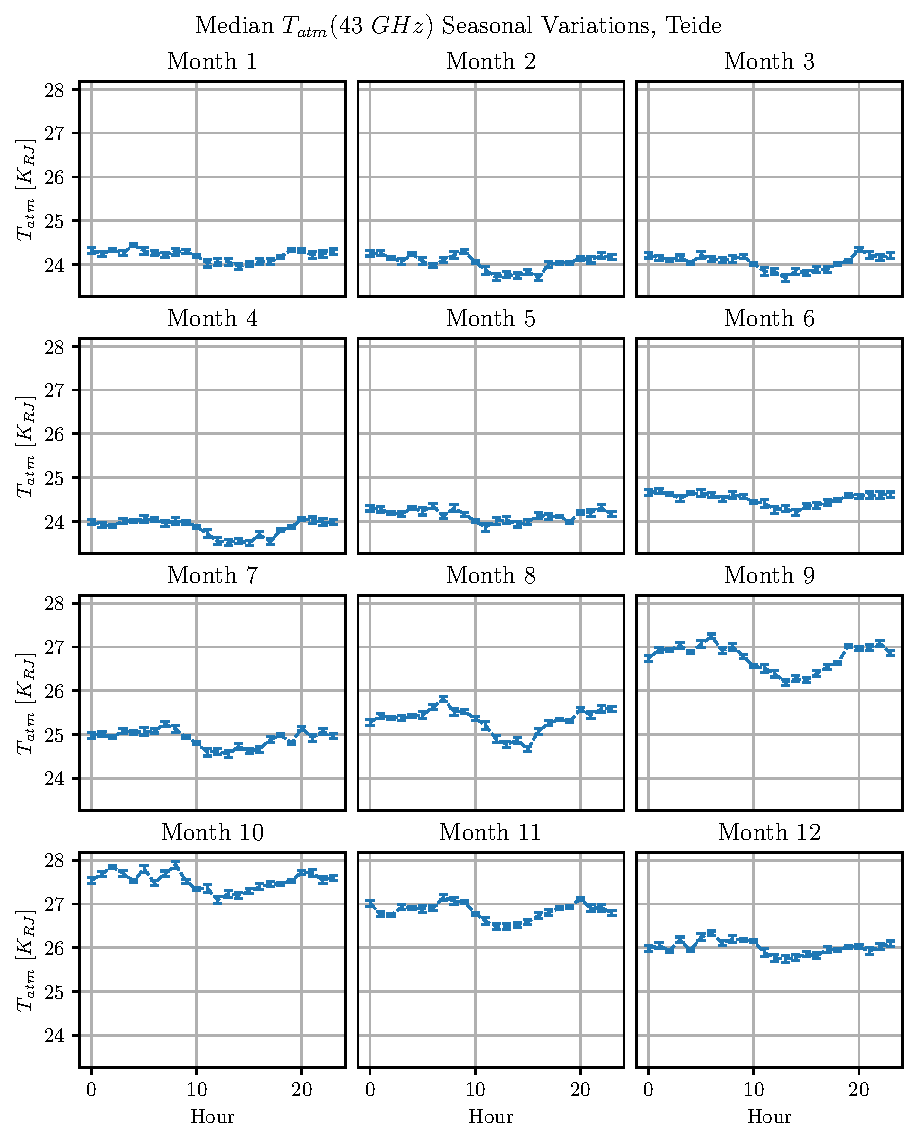
\includegraphics[width=\textwidth]{TATM_nocal}
        \caption{Median atmospheric brightness temperature seasonal
        variations at \SI{43}{\giga\hertz} for Pico del Teide.}
        \label{fig:tatm_nocal}
\end{figure}

\begin{figure}
        \centering
        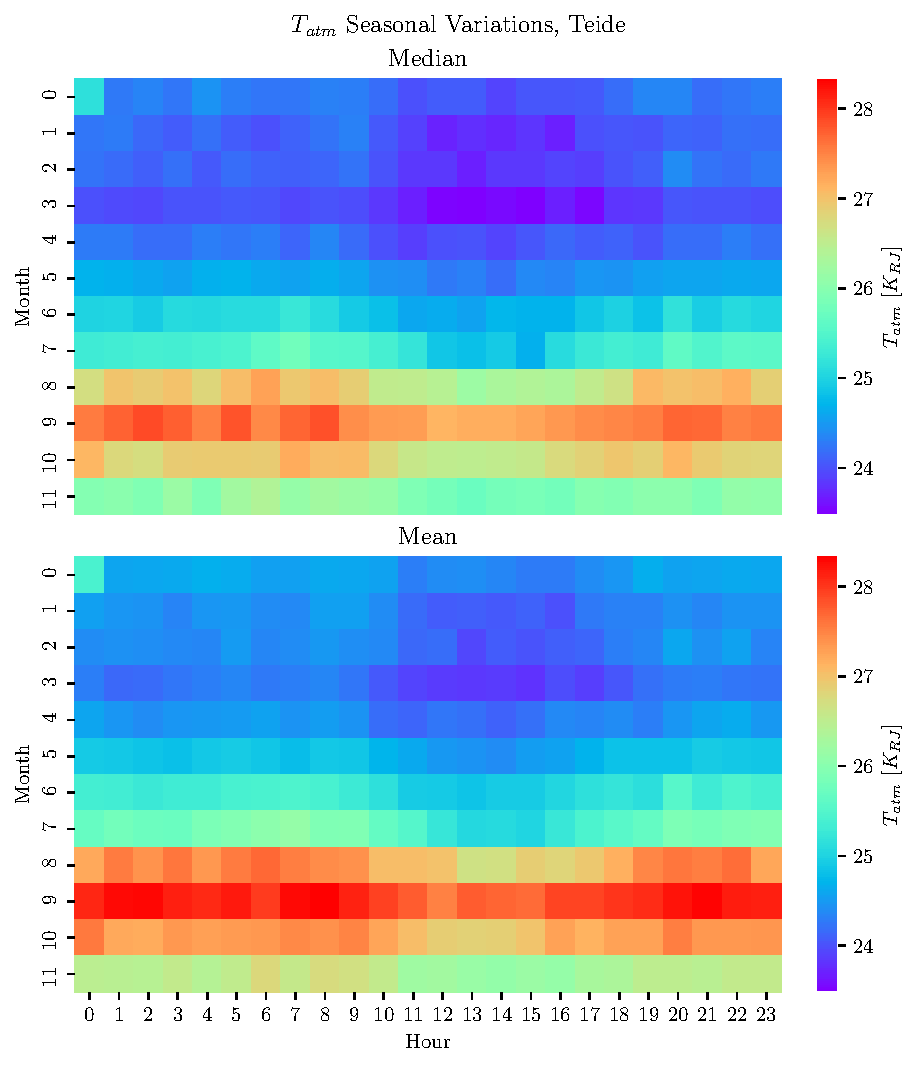
\includegraphics[width=\textwidth]{TATM_Matrices_nocal}
        \caption{$T_\text{atm}$ seasonal matrices at \SI{43}{\giga\hertz}
        for Pico del Teide.}
        \label{fig:tatm_matrices_nocal}
\end{figure}


\chapter{Comparison with QUIJOTE-MFI Data}\label{ch:comparison_quijote}

In this chapter we compare values of atmospheric brightness temperature,
which we have obtained making use of the numerical methods described in
\autoref{ch:statistical_picture} and \autoref{ch:atm_variations}, with
measurements acquired by the QUIJOTE experiment.

In particular, we consider the values of $T_\text{atm}$ that have been measured by the
\emph{Multi-Frequency Instrument} (MFI). MFI is mounted on
the QT1 telescope, which is deployed at the Observatorio del Teide. It
operates since November 2012 in four bands centered at
\SIlist{11;13;17;19}{\giga\hertz}.

\section{QUIJOTE Data and Raw Simulations}

The QUIJOTE dataset is represented in \autoref{fig:quijote_dataset}.  It
includes measurements from a total of \num{444} MFI \emph{sky-dip}
observations, performed between December 2012 and February 2015. Sky-dip
observations are measurements of atmospheric emission performed scanning
the sky at variable elevations. On average, we have one observation every
\num{1.78} days. However, the time distribution of the data is quite
inhomogeneous. There are periods in which we have one observation every
sidereal day (sometimes two per day), but there are some extended periods
without observations.

\begin{figure}
        \centering
        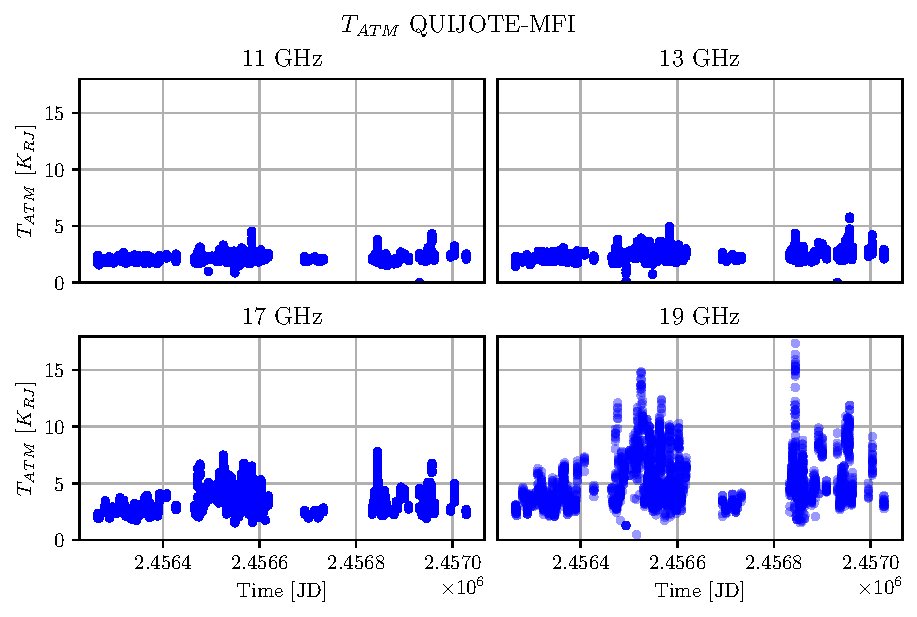
\includegraphics[width=\textwidth]{QUIJOTE_Dataset}
        \caption{QUIJOTE-MFI  $T_{atm}$ dataset.}
        \label{fig:quijote_dataset}
\end{figure}

For each point of the scatter plot showed in \autoref{fig:quijote_dataset},
we have used CAL to simulate a value of atmospheric brightness temperature
at the same frequency and at the same hour of a typical day of the
corresponding month. The comparison between simulated data and
$T_\text{atm}$ acquired by the QUIJOTE-MFI instrument is shown in
\autoref{fig:quijote_sim}.

\begin{figure}
        \centering
        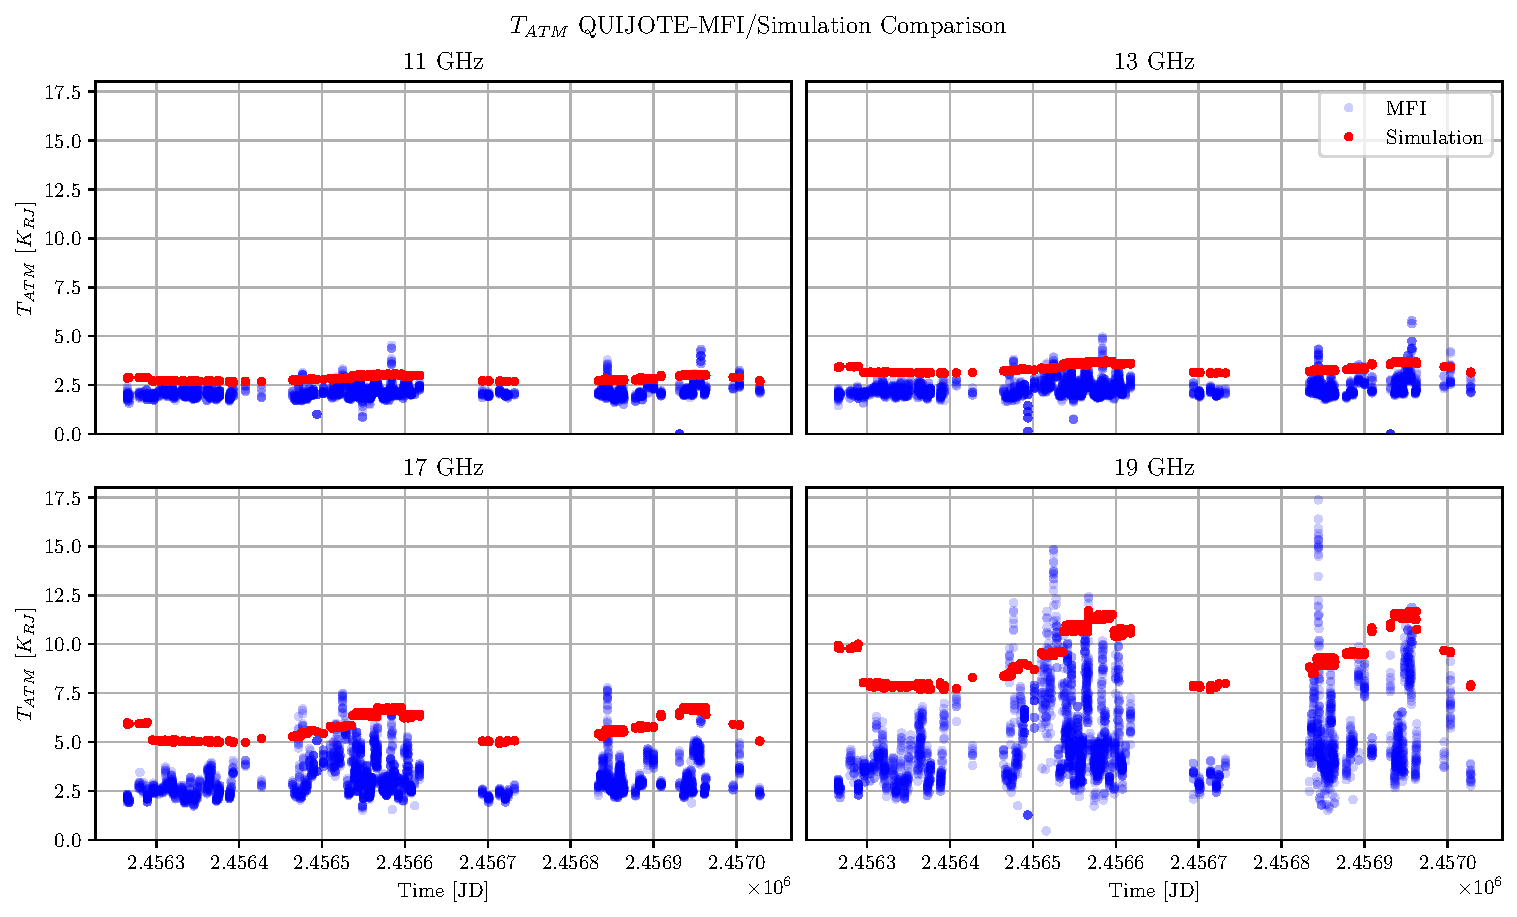
\includegraphics[width=\textwidth]{QUIJOTE-Sim}
        \caption{Comparison between QUIJOTE-MFI measurements and CAL
        simulated data.}
        \label{fig:quijote_sim}
\end{figure}

The scatter plot shows that a significant mismatch occurs. In particular
the simulations performed with CAL, making use of ERA5 dataset, yield
higher values of atmospheric brightness temperature. The mismatch is larger
at higher frequencies, approaching the \SI{22}{\giga\hertz} water vapour
line. Moreover, the QUIJOTE-MFI data exhibit larger fluctuations in time.

We recognise that part of the issues shown in \autoref{fig:quijote_sim}
are due to the insufficient spatial resolution of ERA5 reanalysis data.
\autoref{fig:pwv_teide_1980-01-01_12-00} shows a focus on the pixel in
which the Observatorio del Teide is located. In particular we are
interested in the area in which the Strip telescope will be deployed, which
in the figure is enclosed in a red circle. The ERA5 dataset only provides a
single value per hour of the PWV for the whole pixel, which constitutes a
spatial average.  Therefore, values of PWV are biased by contributions from
coastal low lands, below \SI{2390}{\meter}, and ocean waters. In other
words, the total column water vapour values that have been taken into
account to evaluate atmospheric brightness temperatures greatly exceeds
true values for Pico del Teide.

\begin{figure}
        \centering
        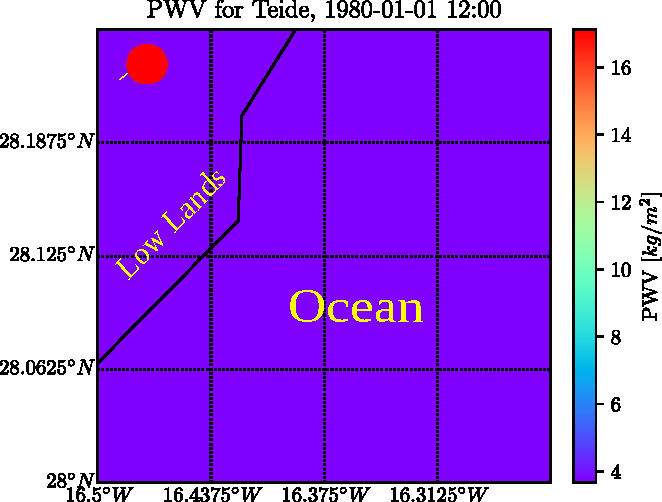
\includegraphics[width=0.80\textwidth]{PWV_Teide_1980-01-01_12-00}
        \caption{PWV for Pico del Teide.}
        \label{fig:pwv_teide_1980-01-01_12-00}
\end{figure}

\section{The Calibration Coefficient}

To mitigate part of the issues presented in the previous section, we have
used atmospheric vertical profiles of $T_s$, $P_s$ and PWV acquired by
balloon probes at Pico del Teide during 2018. These vertical
profiles reflect the true weather conditions near the observation site,
but are characterized by low temporal resolution. This is because balloon
probes need approximately \num{12} hours to measure a whole atmospheric
vertical profile. Therefore, no more than two vertical profiles per day can
be acquired.


The free and open source computer program \emph{Atmospheric Model}
(AM)\footnote{\url{https://zenodo.org/record/3406483}}
\autocite{paine2012atmospheric} has been used to compute sky brightness
temperatures starting from the  median annual vertical atmospheric profile
for the year 2018. AM is a tool for radiative transfer computations at
microwave to submillimeter wavelengths.  Spectra which can be computed with
AM include thermal emission, absorption, transmission, and excess delay.
Median annual values of $T_\text{sky}$ has been obtained in the frequency
range from \SIrange{10}{50}{\giga\hertz}, with a frequency step of
\SI{0.1}{\giga\hertz}.

To compare this result with sky brightness temperatures from CAL,
statistical populations of \num{2736000} elements for the relevant
meteorological parameters have been computed. As before, we have
initialized the \texttt{Weather} method with the CDFs \texttt{.fits} file
for Pico del Teide. The extracted values of PWV, $T_s$ and $P_s$, which are
shown in \autoref{fig:teide_annual_distributions}, are homogeneously
distributed among the months of the year and the hours of the day.
Expectation values for the meteorological parameters were computed from the
corresponding statistical populations using the same estimator choosen for
balloon vertical profiles. The annual median values and corresponding
standard errors for PWV, $T_s$ and $P_s$ are presented in
\autoref{tab:median_meteo_cal}.  These values have been used as input for
the \texttt{atm\_atmospheric\_loading} function to attain values of $T_\text{sky}$
in the appropriate frequency range.

\begin{figure}
        \centering
        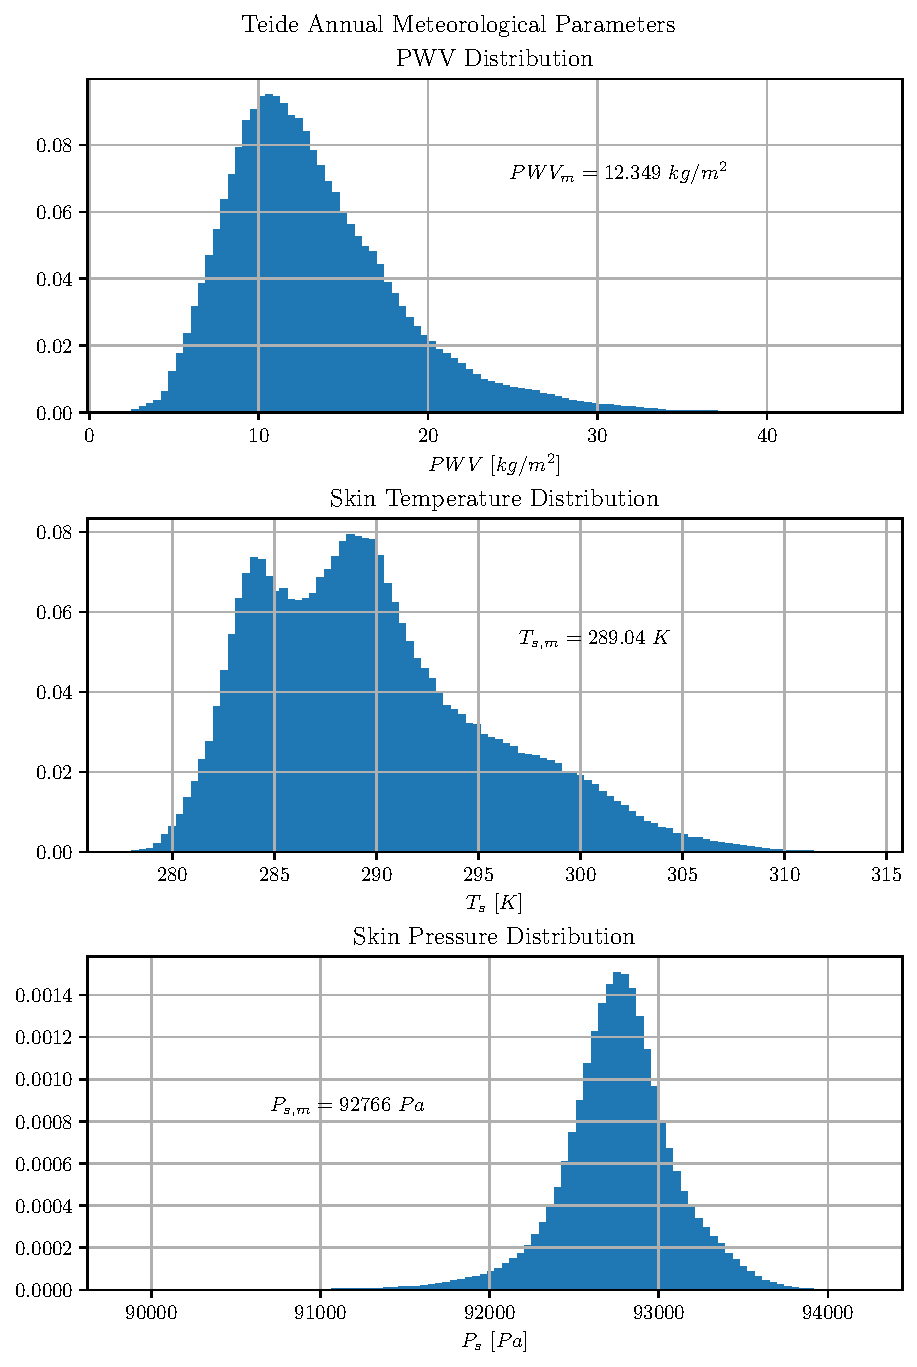
\includegraphics[width=0.93\textwidth]{Teide_Annual_Distributions}
        \caption{Annual distribution for relevant meteorological parameters
        at Pico del Teide obtained using CAL and ERA5 data.}
        \label{fig:teide_annual_distributions}
\end{figure}

\begin{table}
        \renewcommand{\arraystretch}{1.5}
        \centering
        \begin{tabular}{p{5cm} r}
                \hline
                Parameter & Median  \\
                \hline
                \hline
                PWV \dotfill & \SI{12.3491 \pm 0.0029}{\kilo\gram\per\square\meter} \\
                $T_s$ \dotfill& \SI{289.0434 \pm 0.0025}{\kelvin} \\
                $P_s$ \dotfill &  \SI{92766.55 \pm 0.21}{\pascal} \\
                \noalign{\smallskip}
                \hline
        \end{tabular}
        \caption{CAL median values of relevant meteorological parameters.}
        \label{tab:median_meteo_cal}
\end{table}

The sky brightness temperatures that have been computed making use of CAL
and AM are plotted as a function of $\nu$ in
\autoref{fig:am_cal_comparison}. As expected, the $T_\text{sky}$
from CAL assumes an higher value than that computed with the AM computer
program, when evaluated at the same
frequency. The distance between the two curves becomes particularly
significant near the \SI{22}{\giga\hertz} water vapour absorption line.

\begin{figure}
        \centering
        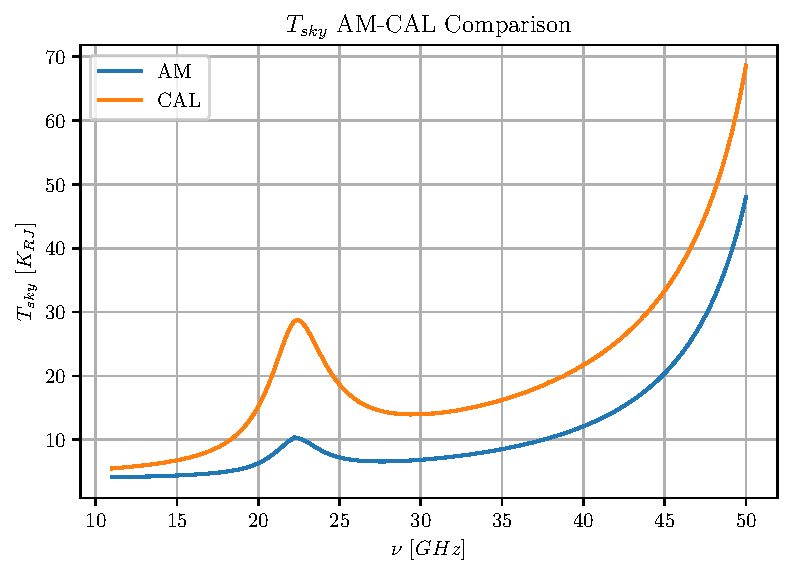
\includegraphics[width=\textwidth]{AM_CAL_Comparison}
        \caption{AM/CAL sky brightness temperatures comparison.}
        \label{fig:am_cal_comparison}
\end{figure}

We can now introduce a calibration coefficient, $k\qty(\nu)$, to correct
higher values in atmospheric brightness temperature computed by CAL, which
are caused by the excess in total column water vapour in ERA5 data for
the pixel in which the observation site is located. The coefficient is defined as

\begin{equation}
        k_\nu \equiv  k\qty(\nu) \equiv
        \frac{T^\text{AM}_\text{atm}\qty(\nu)}{
        T^\text{CAL}_\text{atm}\qty(\nu)}
\end{equation}

It must be noted that $k_\nu$ is assumed to be time independent. This means
that we think that weather conditions are homogeneous across the pixel, and
non-homogeneity in meteorological parameters at a fixed time only depends
on quantities which are not time dependent, such altitude and distance from
the ocean. This assumption could be veriefied acquiring multiple vertical
profiles simultaneously in the same pixel or performing radar scans of the
distribution of clouds and precipitations. The calibration coefficient as a
function of frequency is shown in
\autoref{fig:calibration_coefficient_quijote}.

\begin{figure}
        \centering
        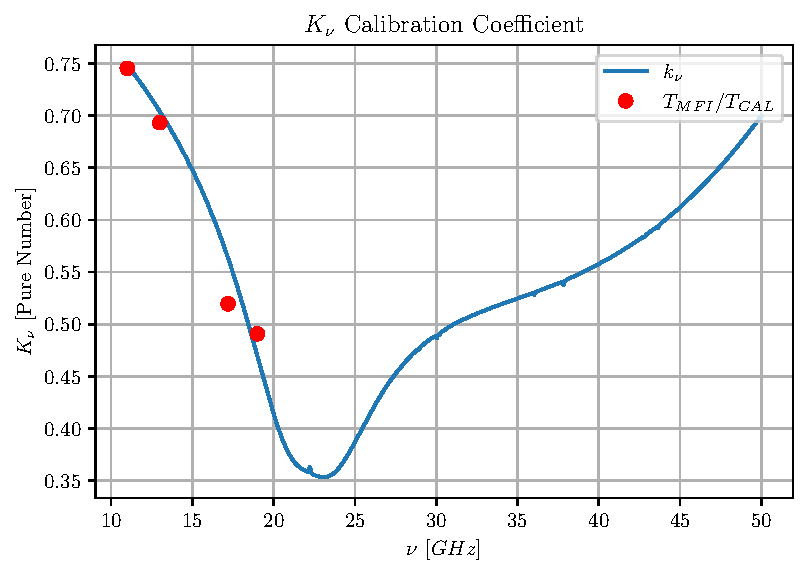
\includegraphics[width=\textwidth]{Calibration_Coefficient_QUIJOTE}
        \caption{$K_\nu$ calibration coefficient.}
        \label{fig:calibration_coefficient_quijote}
\end{figure}

The red dots in the figure represent the ratios between the median values of
atmospheric brightness temperatures measured by QUIJOTE-MFI and those of data
simulated with CAL. As it can be seen, they stand in proximity of the
blue line, confirming the validity of the calibration technique at least
for the MFI central frequencies.

\section{QUIJOTE Data and Calibrated Simulations}

The calibration coefficient defined in the previous section can be used to
correct \autoref{eq:tatm_formula}, which have been employed to calculate
atmospheric brightness temperatures with CAL:

\begin{equation}
        T_\text{atm}\qty(\nu) = k\qty(\nu)\qty[T_\text{sky}\qty(\nu) -
        T_\text{CMB}\qty(\nu)e^{-\tau_A\qty(\nu)}].
        \label{eq:tatm_formula_calibrated}
\end{equation}

\autoref{fig:quijote_sim_calibrated} shows the same comparison that has
been presented in \autoref{fig:quijote_sim}, but atmospheric brightness
temperatures obtained using \autoref{eq:tatm_formula_calibrated} are now
included. At a first glance, the calibrated simulations appear to be
compatible with QUIJOTE-MFI measurements.
\autoref{fig:quijote_sim_calibrated_residuals_boxplot} represents the
boxplot of the residuals for each frequency channel. The expectation values
of the distributions of residuals are compatible with zero for every
frequency within a \SI{95}{\percent} confidence level.

\begin{figure}
        \centering
        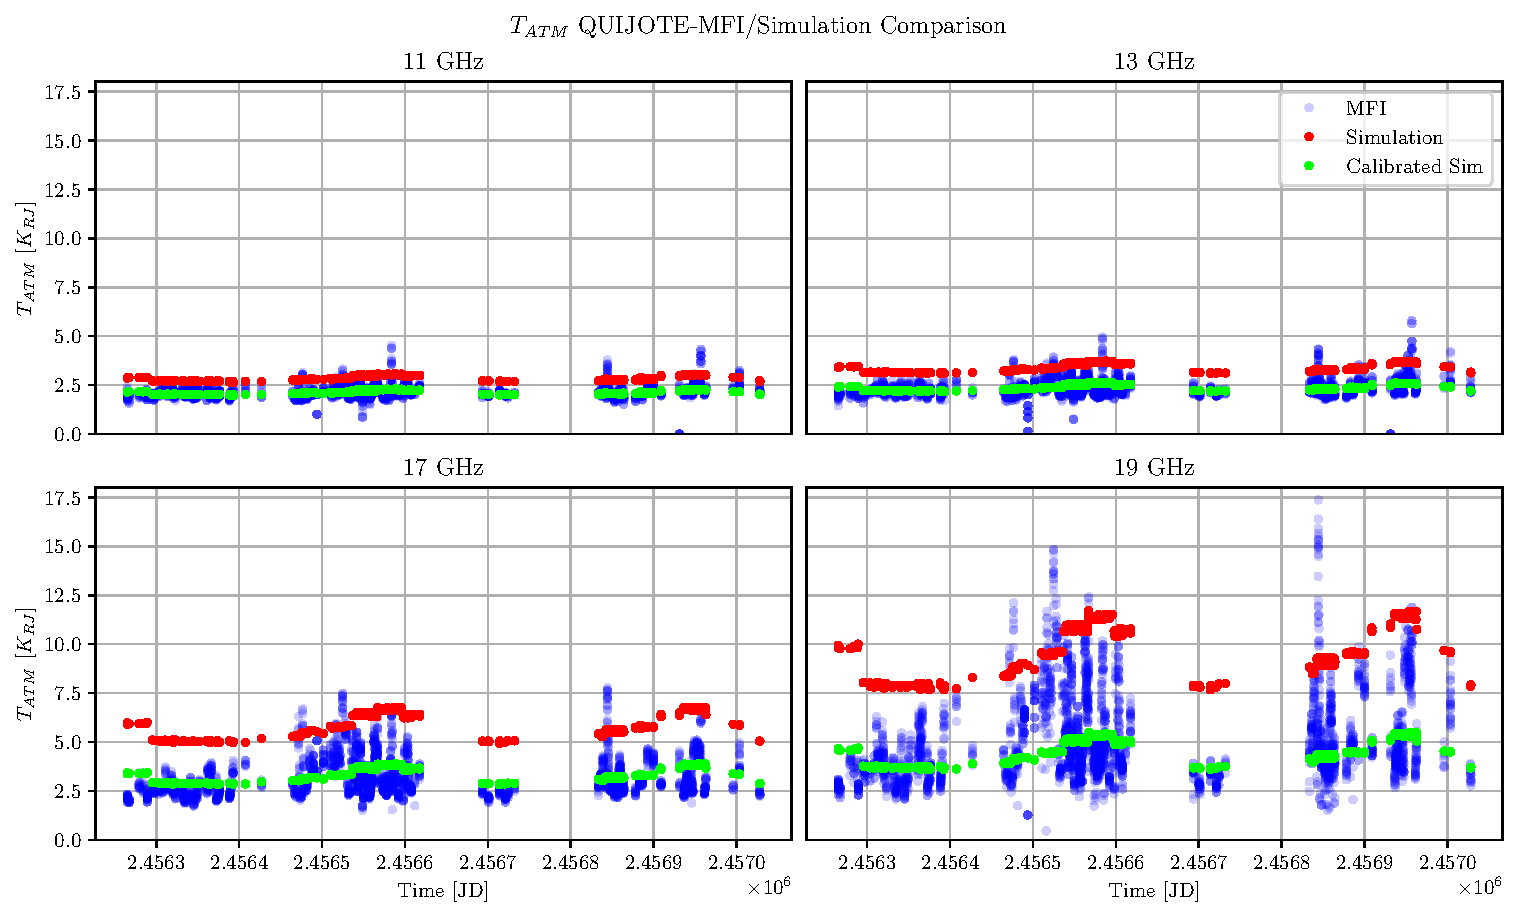
\includegraphics[width=\textwidth]{QUIJOTE-Sim_calibrated}
        \caption{Comparison between QUIJOTE-MFI measurements and
        CAL simulated data with calibration applied.}
        \label{fig:quijote_sim_calibrated}
\end{figure}

\begin{figure}
        \centering
        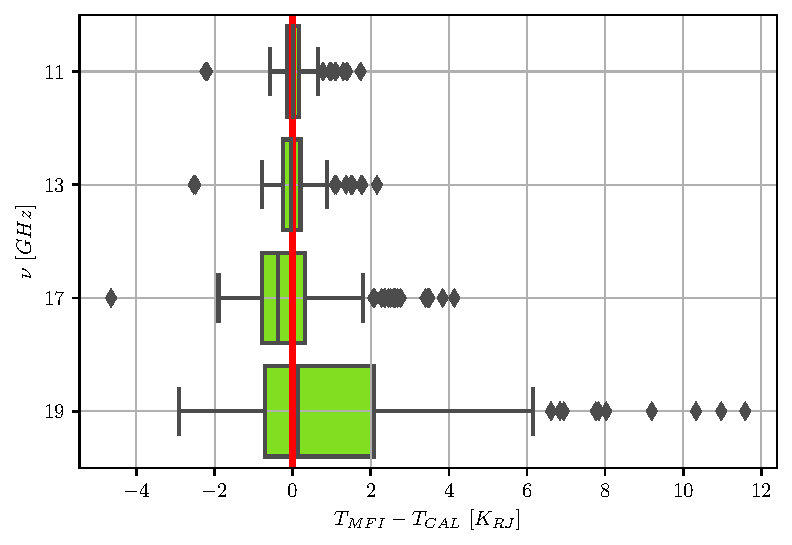
\includegraphics[width=0.93\textwidth]{QUIJOTE-Sim_calibrated_residuals_boxplot}
        \caption{Residuals for QUIJOTE-MFI measurements and
        CAL simulated data with calibration applied.}
        \label{fig:quijote_sim_calibrated_residuals_boxplot}
\end{figure}

However, our simulations can not reproduce fluctuations in atmospheric
brightness temperature and asymmetry in its distribution, which are
observed in particular for the \SI{19}{\giga\hertz} channel.  These
features appear to be more relevant for higher frequencies, approaching the
\SI{22}{\giga\hertz} water vapour absorption line. This suggests that the
dispersion in brightness temperature could be caused by the turbulent
structure of water vapour in the atmosphere, which has been discussed in
\autoref{ss:turbulent_structure}. It's easy to identify the white noise
contribution of the atmosphere at 19 GHz, but the presence of atmospheric
brightness fluctuations indicates that the atmosphere, at higher frequency,
is very complicated to model and the effects of the turbulent structures of
the water vapor are significant.  In conclusion, we can
estimate the average white noise contributions of the atmosphere but there
is another correlated contribute left to figure out.

\chapter{Atmosphere White Noise Contribution}

\section{Strip Polarimeters}

\section{Bandshape Integration}

\chapter{Conclusions}

In this chapter the final results of this master thesis are presented.

The results of a forecast of atmospheric effects for the LSPE/Strip
instrument is presented first. Then, future prospects following this work
are given.

\section{A Forecast for the LSPE/Strip Instrument}

Using the methods discussed in \autoref{ch:comparison_quijote}, we have
produced a forecast of the seasonal variations of atmospheric
brightness temperature for the Q-band of the Strip instrument of the LSPE
experiment, at \SI{43}{\giga\hertz}. The Strip telescope is briefly
Described in \autoref{ch:lspe_strip}.

We have calculated a population of atmospheric brightness temperatures for each
hour of the typical day of each month of the year, using CAL. As usual, the
\texttt{Weather} class has been initialized with the CDF \texttt{.fits}
file for Pico del Teide. Every statistical population contains exactly
\num{9900} elements. The expectation values of each population and the
corresponding standard errors has been obtained, using median as estimator.
As before, standard errors have been computed splitting the statistical
populations in \num{10} samples of the same number of elements and
applying a bootstrapping technique.

\autoref{fig:tatm_cal} shows the annual variations of
$T_\text{atm}\qty(\SI{43}{\giga\hertz})$ and the corresponding standard
errors. Instead, \autoref{fig:median_tatm_matrix_cal} represents the same
data in a color map. Several pieces of information can be extracted from
these graphs.

\begin{figure}
        \centering
        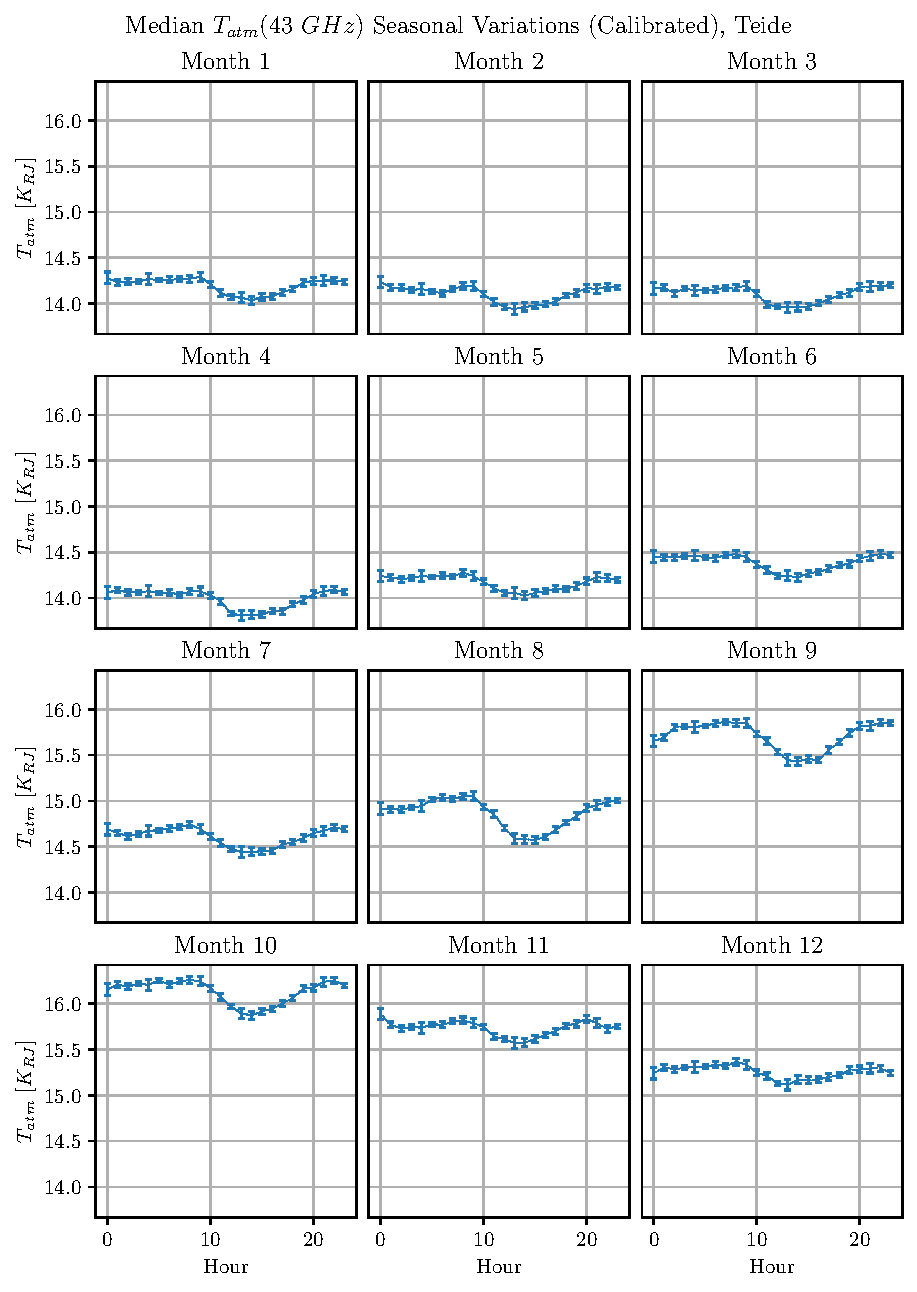
\includegraphics[width=0.96\textwidth]{TATM_cal}
        \caption{Median seasonal variations of atmospheric brightness
        temperature at \SI{43}{\giga\hertz} for Pico del Teide. Error bars
        have been tripled in size to make them more visible.}
        \label{fig:tatm_cal}
\end{figure}

\begin{figure}
        \centering
        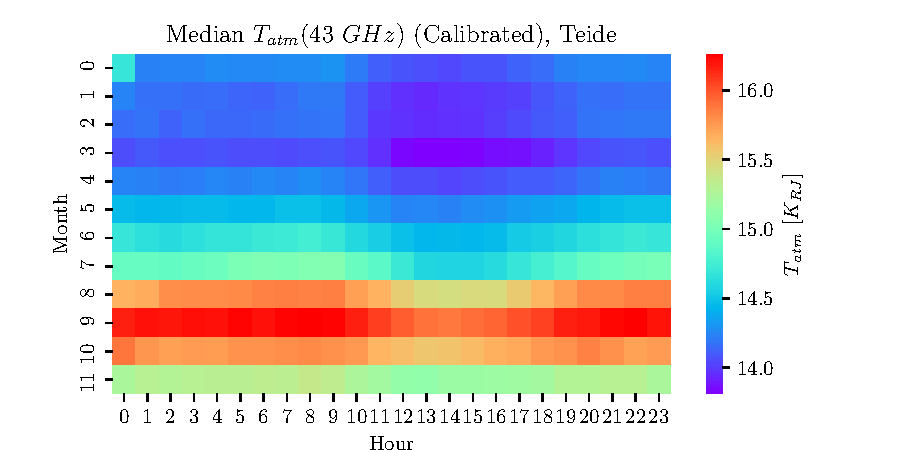
\includegraphics[width=\textwidth]{Median_TATM_Matrix_cal}
        \caption{Seasonal matrix for median atmospheric brightness
        temperature at \SI{43}{\giga\hertz} for Pico del Teide.}
        \label{fig:median_tatm_matrix_cal}
\end{figure}

\autoref{tab:mean_tatm_month} contains average atmospheric brightness
temperatures at \SI{43}{\giga\hertz} and the corresponding errors for each
month of the year. We have obtained these values averaging the data of each
month over the hours of the day. As we can see, the extra loading of the
atmosphere on the detectors is maximum in October and in general assumes
values over $3\sigma$ above its annual average of \SI{14.77 \pm
0.21}{\kelvin} in September, October and November. In fact, these months
are characterized by great values of PWV, as we can learn from
\autoref{fig:teide_seasonal_matrices_vertical}.

\begin{table}
        \renewcommand{\arraystretch}{1.5}
        \centering
        \begin{tabular}{p{5cm} r}
                \hline
                Month & Average $T_\text{atm}\qty(\SI{43}{\giga\hertz})\
                \qty[\si{\kelvin}]$ \\
                \hline
                \hline
                Gen \dotfill & \num{14.198 \pm 0.017} \\
                Feb \dotfill & \num{14.106 \pm 0.018} \\
                Mar \dotfill & \num{14.107 \pm 0.017} \\
                Apr \dotfill & \num{13.991 \pm 0.021} \\
                May \dotfill & \num{14.169 \pm 0.016} \\
                Jun \dotfill & \num{14.390 \pm 0.018} \\
                Jul \dotfill & \num{14.608 \pm 0.020} \\
                Aug \dotfill & \num{14.865 \pm 0.032} \\
                Sep \dotfill & \num{15.707 \pm 0.031} \\
                Oct \dotfill & \num{16.131 \pm 0.026} \\
                Nov \dotfill & \num{15.733 \pm 0.017} \\
                Dec \dotfill & \num{15.256 \pm 0.014} \\
                \noalign{\smallskip}
                \hline
        \end{tabular}
        \caption{Monthly average atmospheric brightness temperature at
        \SI{43}{\giga\hertz} for Pico del Teide.}
        \label{tab:mean_tatm_month}
\end{table}

\autoref{tab:mean_tatm_dayly_esc} displays the average daily excursion of
atmospheric brightness temperature for each month of the year. We have used
an analogous approach to that described above for average $T_\text{atm}$s to
obtain these values. The daily excursion is maximum in August and in
general it takes values over $3\sigma$ above its annual average of
\SI{0.312 \pm 0.023}{\kelvin} in the months of August, September and
October. Again, from \autoref{fig:teide_seasonal_matrices_vertical} we
learn that these are the months of the year in which surface pressure
takes its greatest values.

\begin{table}
        \renewcommand{\arraystretch}{1.5}
        \centering
        \begin{tabular}{p{5cm} r}
                \hline
                Month & Average $\Delta
                T_\text{atm}\qty(\SI{43}{\giga\hertz})$
                Day [\si{\kelvin}] \\
                \hline
                \hline
                Gen \dotfill & \num{0.258 \pm 0.022} \\
                Feb \dotfill & \num{0.296 \pm 0.015} \\
                Mar \dotfill & \num{0.240 \pm 0.017} \\
                Apr \dotfill & \num{0.284 \pm 0.016} \\
                May \dotfill & \num{0.250 \pm 0.013} \\
                Jun \dotfill & \num{0.253 \pm 0.017} \\
                Jul \dotfill & \num{0.301 \pm 0.022} \\
                Aug \dotfill & \num{0.479 \pm 0.023} \\
                Sep \dotfill & \num{0.434 \pm 0.022} \\
                Oct \dotfill & \num{0.387 \pm 0.033} \\
                Nov \dotfill & \num{0.314 \pm 0.030} \\
                Dec \dotfill & \num{0.251 \pm 0.014} \\
                \noalign{\smallskip}
                \hline
        \end{tabular}
        \caption{Average daily excursion of atmospheric brightness
        temperature for Pico del Teide at \SI{43}{\giga\hertz} for each
        month.}
        \label{tab:mean_tatm_dayly_esc}
\end{table}

Instead, the average annual excursion of atmospheric brightness temperature
can be obtained from \autoref{tab:mean_tatm_month}. It takes a value of
\SI{2.139 \pm 0.033}{\kelvin}, showing that the extra load on detectors
from atmospheric effects is subjected to relatively small daily variations
as compared to overall annual variations.

The findings presented in this section can be used as a starting point to
forecast the maximum sensitivity that Strip radiometers can reach due to
atmospheric effects.  We show some preliminaries results in
\autoref{sensitivity}.

\section{Future Prospects}

The statistical model of atmospheric emission that we have presented in
this master thesis is just the starting point to provide a complete
representation of the atmosphere in the microwaves range. More
meteorological parameters, such as wind speed components, total column
liquid water and total column ice water, can and must be taken into account
in order to describe the atmospheric turbulent structure and to evaluate
the resulting correlated noise contribution.

Our CDFs \texttt{.fits} file already includes the whole set of useful
meteorological parameters. In addition, the CMB atmospheric library already
implements the Kolmogorov-Taylor model for atmospheric turbulence.
Therefore, we are confident that time ordered data simulations of
atmospheric emission for the LSPE/Strip telescope, or any other
instruments, could be successfully obtained in future works.


\backmatter

\end{document}
